\documentclass[11pt]{article}
\pdfoutput=1
\usepackage{jcappub}
\usepackage{aas_macros}
\usepackage{graphics,graphicx, url}
\usepackage{amsmath,amssymb}
\graphicspath{{figures/}}
\def \figwidth{0.8\textwidth}
\def \halffigwidth{0.48\textwidth}
\begin{document}

\title{Primordial Power Spectra Reconstruction Constrained by a Measured Tensor Amplitude}
\author[a]{J. Richard Bond}
\author[a,b]{Jonathan Braden}
\author[c]{Andrei Frolov}
\author[a]{Zhiqi Huang}
\author[d]{Pascal Vaudrevange}
\affiliation[a]{CITA}
\affiliation[b]{Dept. of Physics, U of T}
\affiliation[c]{Simon Fraser University}
\affiliation[d]{Germany}

\emailAdd{bond@cita.utoronto.ca}
\emailAdd{jbraden@cita.utoronto.ca}
\emailAdd{frolov@sfu.ca}
\emailAdd{zqhuang@cita.utoronto.ca}

\abstract{The shapes of the primordial scalar power spectra are the key quantities to unravel the physics of the inflationary epoch. Blahblah...}

\date{\today}
\maketitle

\section{Introduction}

The cosmic microwave background radiation is a unique window into the physics of energy scales above TeV. Progress towards harvesting its information content has been steady on the experimental side, starting with the COBE experiment \cite{COBE1996}, continuing with balloon borne experiments such as Boomerang \cite{Boomerang2001, Boomerang2003}, ground-based experiments such as ACT \cite{ACT2013, ACT2014}, SPT \cite{SPT2013, SPT2014} and BICEP \cite{BICEP2}, and the satellites WMAP \cite{WMAP9Maps, WMAP9Cosmology} and Planck \cite{Planck2013Overview, Planck2013PowerSpectra, Planck2013Parameters}. They delivered a picture of a universe that is extremely homogeneous: Gaussian fluctuations sit on top of a uniform background of photons that stream to us from the surface of last scattering at redshift about $1100$, with an amplitude of about $10^{-5}$. Decomposing this image of the microwave sky into spherical harmonics shows an angular power spectrum whose features are well understood. Acoustic oscillations in the primordial photon-baryon fluid freeze out at the surface of last scattering, with the photons streaming (almost) freely towards us, showing the familiar acoustic peaks in the angular power spectrum. Their locations and relative amplitudes allow us to infer the energy content of the universe.

While experimental advances have been formidable, the exact properties of microscopic theories responsible for the inflationary period remain elusive. A plethora of different scalar field potentials have been suggested, and many of them are compatible with current observations. From a theoretical perspective, the best that can be said is that there are many scalar fields in string theory. As for their potentials, not much is known. Even though some advances have been made in building models of inflation based on or inspired by string theory \cite{KKLT, Blanco-Pillado:2004ns, Blanco-Pillado:2006he, KKLMMT, CQ, GKP, Silverstein:2008sg}, the vast majority of the string landscape is still unchartered.


Traditionally the inflationary dynamics are described in the slow-roll approximation, assuming that the inflaton field rolls slowly (or with small acceleration) down its potential. For the simplest single-field slow-roll models, both the scalar and tensor power spectra are very close to power-law and the tilt of tensor power spectrum satisfies a consistency-relation. As a consequence, as far as only observables are concerned, these models can be described with three parameters: the amplitude of the scalar power spectrum ($A_s$), the tilt of the scalar power spectrum ($n_s-1$), and the tensor-to-scalar ratio ($r \equiv A_T/A_s$ where $A_T$ is the amplitude of tensor power spectrum). The tilt of the tensor power spectrum, according to slow-roll approximation, is $n_t = -r/8$. 


Thanks to the plethora of observational data that are already available today, we can go beyond the simplest models and ask whether a single-field slow-roll model is adequate to describe the data. To answer such a question it is necessary to extend the parameter space with reasonable theoretical motivations. For a broad class of models, the tensor power spectrum remains to be a power-law with a small tilt. This is because the tensor power spectrum, almost model-independently, only depends on the energy scale of inflation, which by definition does not vary much. Observationally, because of the smallness of $B$-mode polarization signature and the limited range of scales where tensor power spectrum can be measured, it is very difficult to measure features in the tensor power spectrum. Thus, it is reasonable to keep the parametrization of tensor power spectrum unchanged. For the future, we might be able to explore the small tilt of tensor power spectrum and test the sinlg-field slow-roll consistency relation. In that case, $n_t$ should be introduced as a free parameter. For the current data, we do not bother to do so as $n_t$ at this stage is far from being measurable to the accuracy of testing the consistency relation. However, while a broader class of inflation models are permitted, the scalar power spectrum, becomes very model-dependent \cite{Linde1996, Starobinsky1998, Lyth2003, Barnaby2009b, Bond2009}. Phenomenologically, back to the early COBE era, a running parameter $n_{\rm run}$ was already introduced as a minimal extension to describe the scale dependence of the tilt of scalar power spectrum \cite{Kosowsky1995}. Theoretically, a tiny running $\lesssim 10^{-3}$ is expected from  single-field slow-roll models. A detectable running $\gtrsim 0.01$ requires a very slow phase-transition over many efolds of inflation, which is not very well motivated. However, if only one or two degrees of freedom are to be added, there is no ``optimal'' or ``universal'' parameterization that can describe a much broader class of models. For this reason, the running parameter remains to be ``the standard extension'' to date. This situation, however, can be changed if we add more degrees of freedom into the parametrization. Because the observable range of cosmological scales is about ten efolds, a function interpolated from about 10 knots can cover most of the features that are not much shaper than one efold in scale. This interpolation method, to be thoroughly explored in this paper, provides an alternative approach to study the primordial power spectra with very little theoretical priors imposed. The philosophy here is to let the data guide our theoretical thoughts.

If we only consider the CMB temperature-temperature (TT) auto-correlation, the immediate problem of allowing an ``arbitrary'' shape of scalar power spectrum is that the tensor contribution to the TT correlation can be mimicked by a scalar power spectrum with a proper shape. There is hence a strong degeneracy between the scalar and tensor power spectra. The theoretical prediction of the amplitude of tensor power spectrum varies from $r\sim 10^{-10}$ for many string-motivated small-field models to  $r\sim 0.1$ for large-field models, with the scales in between almost all plausible. Thus, this degeneracy cannot be relieved by imposing a theoretical prior. We need additional data to constrain the tensor power spectrum independently. The recent detection of B-mode polarization in CMB \cite{BICEP2}, although remains to be confirmed by other experiments, casts a light on solving this problem. 

This paper is structured as follows. Blahblah...The reduced Planck mass is denoted as $M_p\equiv 1/\sqrt{8\pi G}$, where $G$ is Newton's gravitational constant.We use FRW metric $ds^2 = -dt^2 + a^2(t) d\mathbf{x}^2$. The Hubble parameter $H$ is defined as $H\equiv \frac{\dot a}{a}$, where a dot represents derivative with respect to the cosmological time $t$.

\section{Reconstructing Primordial Trajectories}

Following the convention in the literarture we use $\Delta^2_{S}(k) \equiv \frac{k^3P_S(k)}{2\pi^2}$ and $\Delta^2_T(k) \equiv \frac{k^3P_T(k)}{2\pi^2}$ to denote the scalar- and tensor power spectra, respectively. These power spectra are $k$-volumed weighed, and are nearly flat for most of the inflation models.

The CMB temperature-temperature angular power spectrum $C_\ell^{TT}$ from tensor contribution with $r=0.2$ (the central value suggested by BICEP2 \cite{BICEP2}) can be generated by an effective scalar power spectrum shown in Figure~\ref{fig:effps}. To avoid this degeneracy between tensor- and scalar contributions, we can either assume $r$ to be some specific value and discuss the constraints on scalar power spectrum under such an assumption, or use BICEP2 data to independently constrain the tensor power spectrum. We will apply both approaches in this section. When fixing $r$ we use fiducial values $r=0.02$,  $0.2$ and $0.5$ as typical examples, whereas for ``free'' $r$ we use a flat prior $0\le r < 1$. The lower bound $r\ge 0$ is defined by theory, while the assumed upper bound $r<1$ does not affect the result as long as it is much higher than the observational upper bound, which, from BICEP2 is about $0.4$ at 99.7\% confidence level.   


\begin{figure}
  \centering
  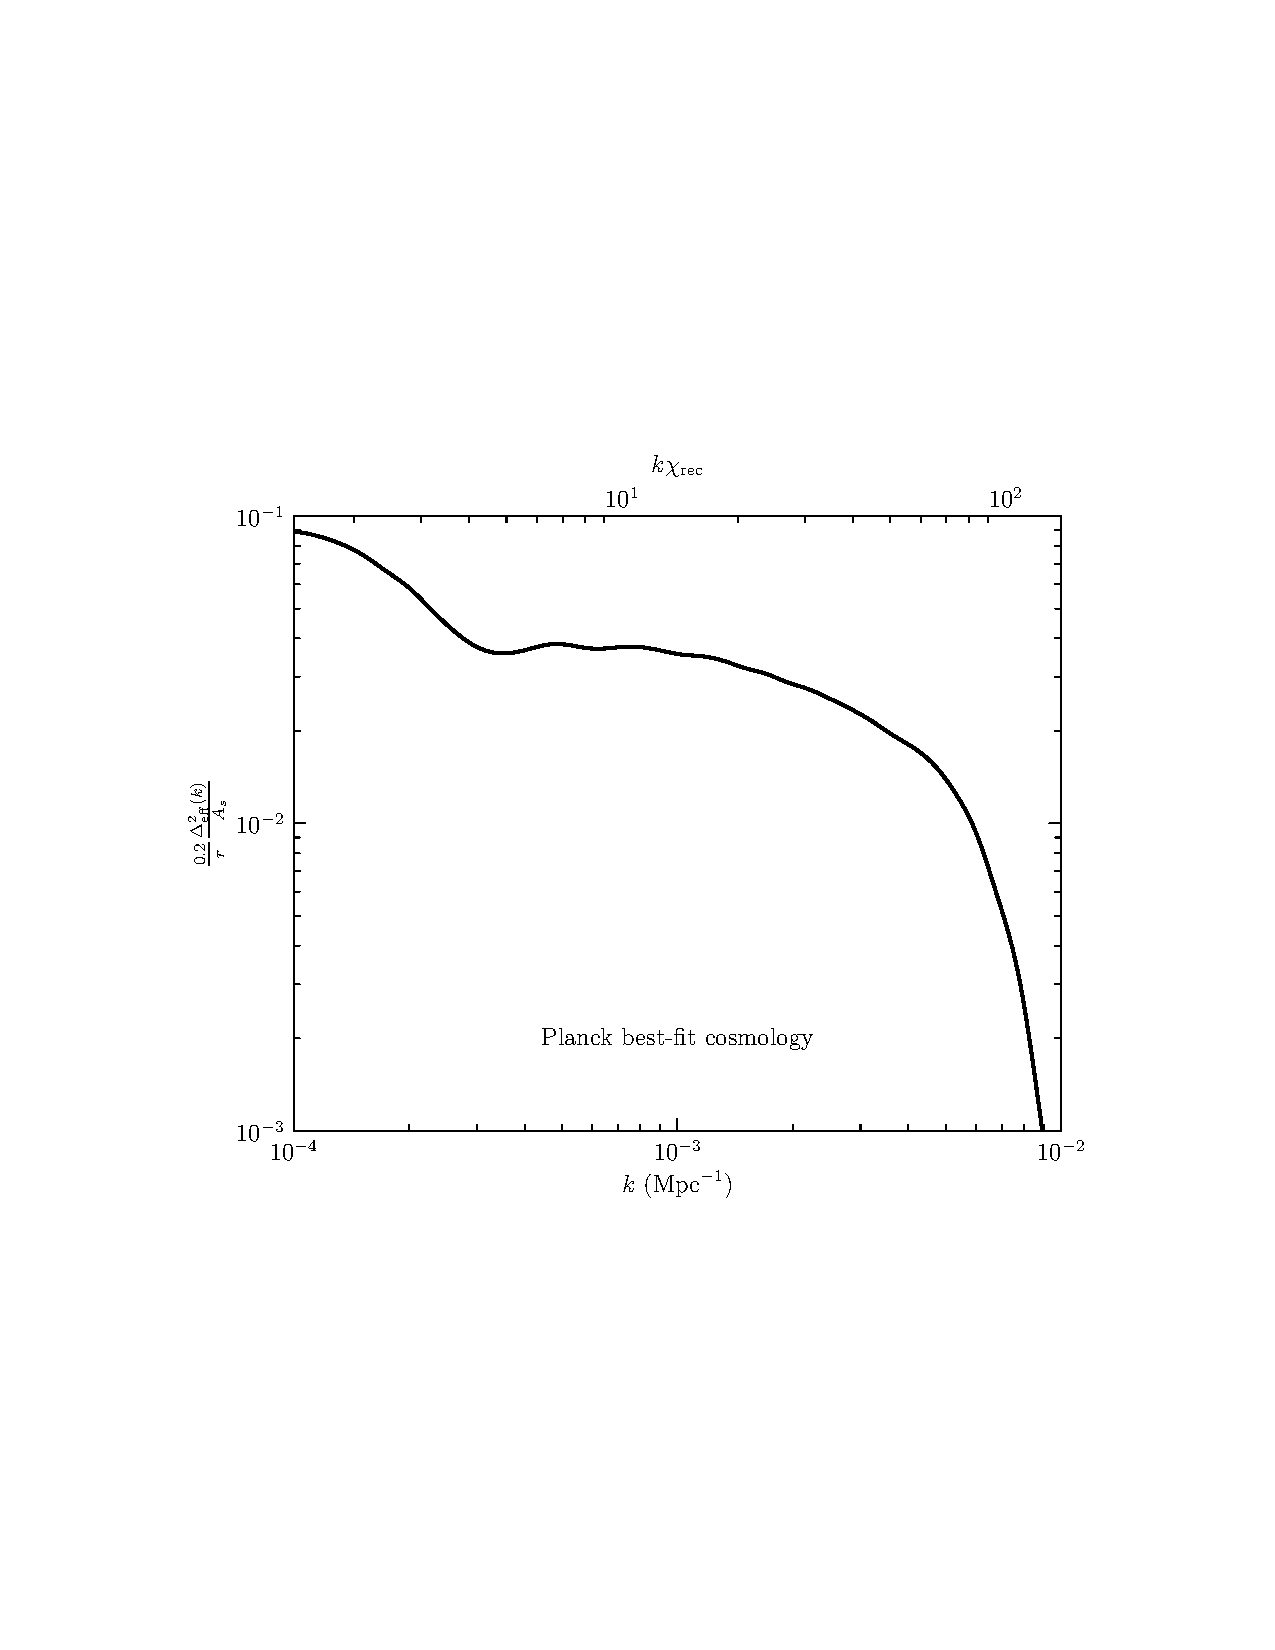
\includegraphics[width = \figwidth]{ten_eff_ps.pdf}
  \caption{The effective scalar power spectrum that produces the same $\Delta C_\ell^{TT}$ contribution as a $r=0.2$ tensor power spectrum would do. Planck best-fit cosmology is assumed. \label{fig:effps}}
\end{figure}


We use the public available software CosmoMC \cite{CosmoMC} to do Monte Carlo Markov Chain (MCMC) calculations. The software is modified to include our parametrization of the primordial power spectra. For the runs with fixed $r$, we use Planck data including lensing (Planck), WMAP polarization (WP), ACT and SPT high-ell data (highL) and Baryon Acoustic Oscillations (BAO) constraint from Sloan Digital Sky Survey (SDSS) \cite{SDSSDR9} and Six-degree-Field Galaxy Survey (6dF) \cite{Jones2004, Jones2009}. The BICEP2 data is used only for runs with $r$ varying. We use 11 knots as a representative case. We verify, by varying the number of knots (typically, from 9 to 15), that the results are not sensitive to the number of knots.

A $n$-knots parametrization is constructed by interpolating scalar power spectrum between $n$ knots. In our parametrization,  $A_s$ is still defined as the amplitude of scalar power sepctrum at $k_{\rm pivot}=0.05 {\rm Mpc}^{-1}$. The knots $k_1$, $k_2$, ..., $k_n$ are uniform in $\ln k$, with $k_{\rm pivot}$ being one of the knots $k_{i_p} = k_{\rm pivot}$ ($i_p$ is a fixed integer between $1$ and $n$). Additional $n-1$ parameters are introduced to describe the deviation from scale-invariance. They are defined as $\gamma_i\equiv \Delta^2_S(k_i)/ A_s$, for $i = 1, 2, \ldots, i_p - 1, i_p+1, \ldots, n$.  The choice of $i_p$ and spacing $\delta\ln k \equiv \ln (k_{i+1}/k_i)$ depends on the number of knots. The criterion is that the relevant cosmological scales (roughly from $10^{-4}{\rm Mpc}^{-1}$ to $0.2 {\rm Mpc}^{-1}$) are covered from $k_1$ to $k_n$. For the MCMC runs we assume flat prior on $\ln A_s$ and $\ln \gamma_i$ ($i\neq i_p$). For scales between $k_1$ and $k_n$, we cubic-spline interpolate $\ln (\Delta^2_S(k)/A_s)$ with natural boundary conditions (second derivatives vanish). Whereas for scales beyond, we simply assume $\Delta^2_S(k) = \Delta^2_S(k_1)$ for $k<k_1$ and $\Delta^2_S(k) = \Delta^2_S(k_n)$ for $k>k_n$. As for the tensor power spectrum, we use a parametrization $\Delta^2_T(k) = r A_s (k/k_{\rm pivot})^{n_t}$ with $n_t = -r/8$ enforced. Note that in the literature $r$ is often defined as the tensor-to-scalar ratio at $k=0.002 {\rm Mpc}^{-1}$, slightly different from the $r$ defined here. We do not adopt this convention because with our parametrization, the scalar power at $k=0.002 {\rm Mpc}^{-1}$ is poorly measured, whereas the conventional parametrization extrapolates the scalar power to all scales with a constant $n_s$. In all the runs we use a prior $-2 \le \ln \gamma_i \le 2$ ($i = 1, 2, \ldots, i_p - 1, i_p+1, \ldots, n$). For most of the knots this prior does not matter, as the data only allow a much narrower range of $\ln \gamma_i$. However, for the superhorizon scales $k\lesssim 10^{-4} {\rm Mpc}^{-1}$ and very small scales $k\gtrsim 0.2 {\rm Mpc}^{-1}$ that are not measured by the cosmological data, the prior will dominate the results. 

In Fig~\ref{fig:traj_power_fixr} we show the reconstructed scalar power spectrum with different fiducial $r$. In the prior dominated scales ($k\le 10^{-4} {\rm Mpc}^{-1}$ and $k\gtrsim 0.2 {\rm Mpc}^{-1}$), the trajectories tend to uniformly scan the allowed prior $-2\le \ln \gamma_i\le 2$. In the observable-scale range, however, the trajectories are not perfectly favoring a power-law shape. They tend to bend down (w.r.t. power-law extrapolation) at $10^{-4} {\rm Mpc}^{-1} \lesssim k \lesssim 0.01 {\rm Mpc}^{-1}$. This tendency is more significant for larger fiducial $r$, because a deficit in scalar power at $k\lesssim 0.01 {\rm Mpc}^{-1}$ is needed to cancel the tensor contribution to $C_\ell^{TT}$. 

\begin{figure}
  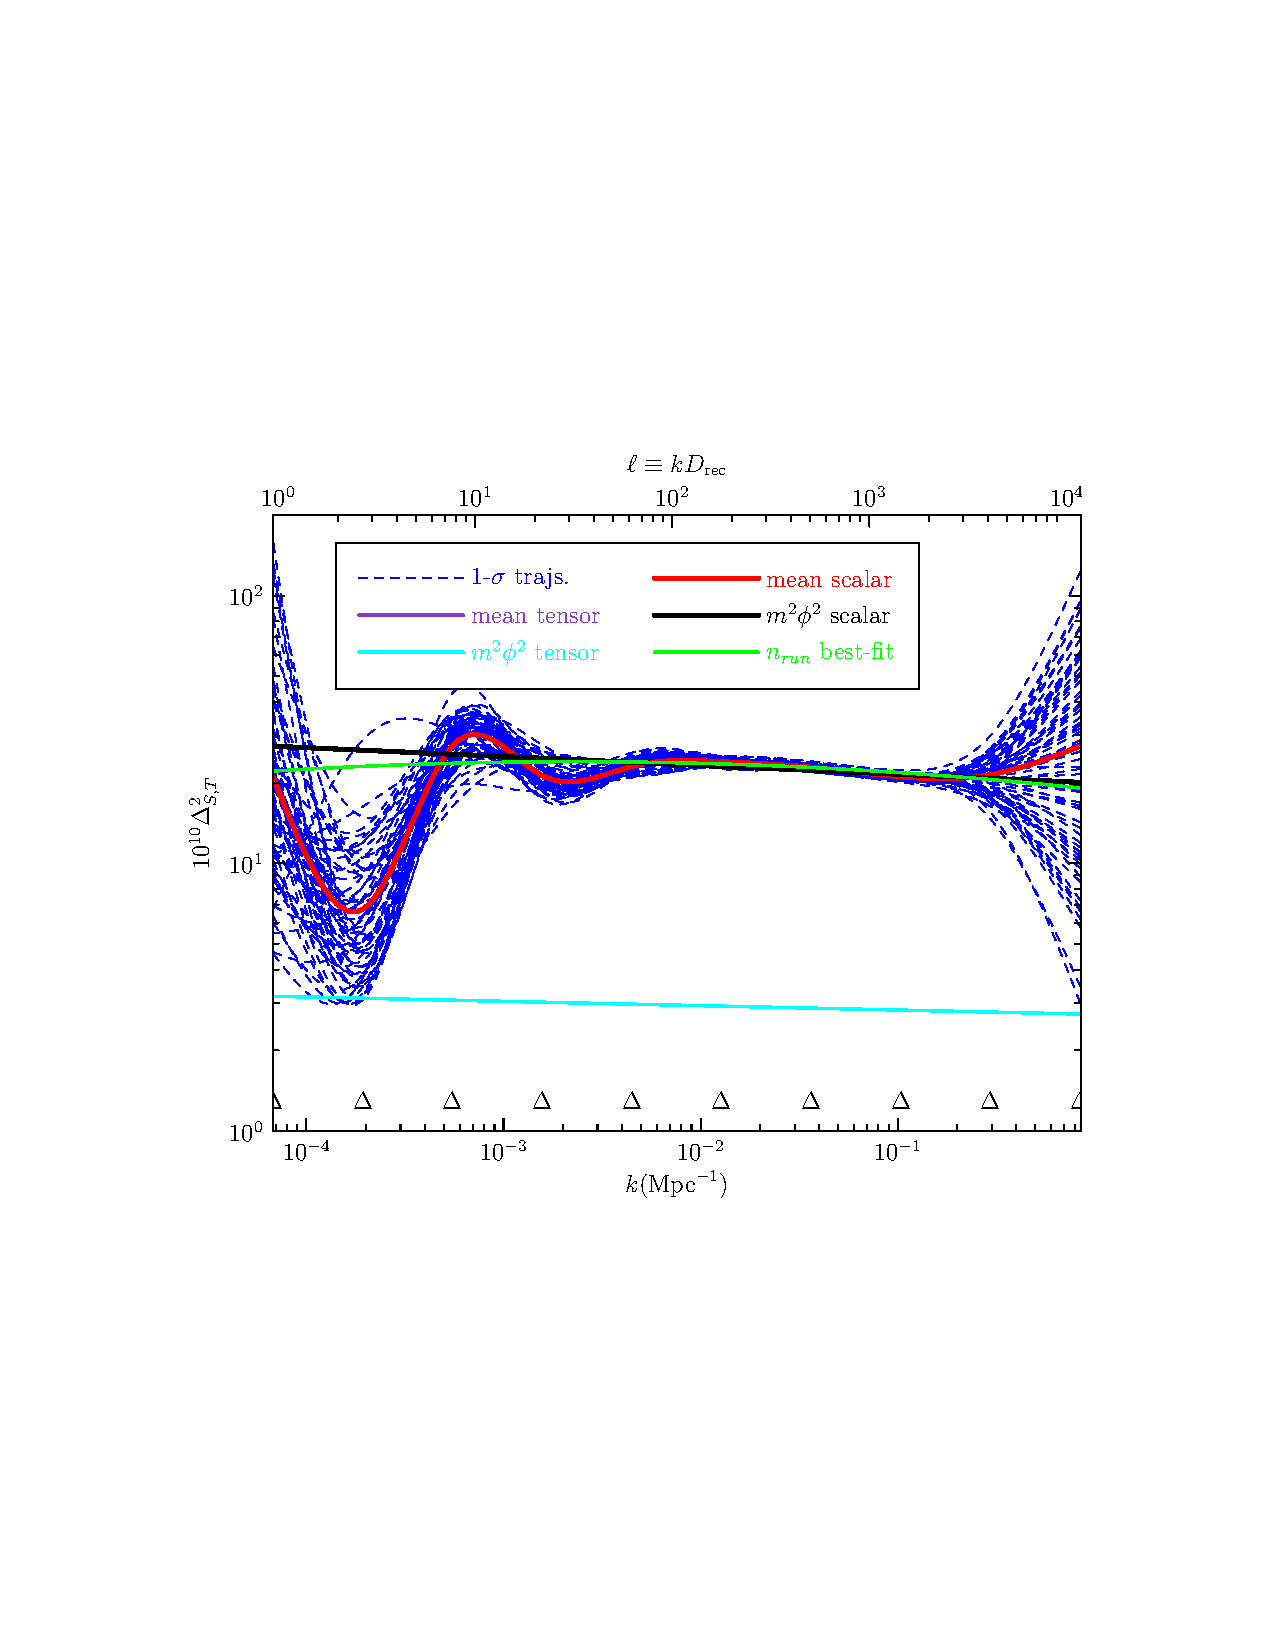
\includegraphics[width=\halffigwidth]{nobicep_spline0_p11_r0d02_power_traj.pdf}% 
  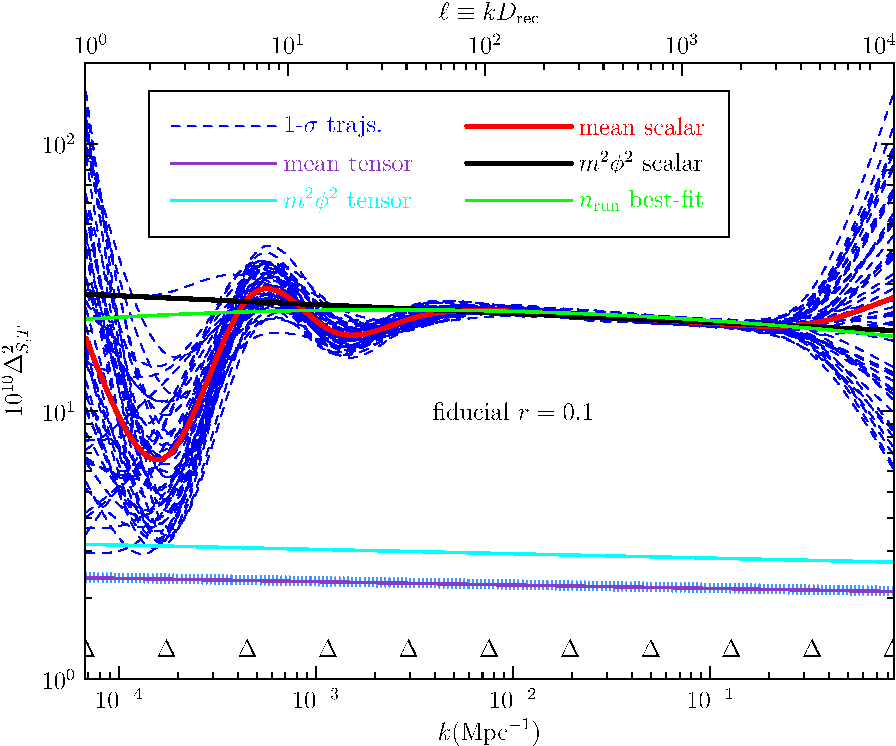
\includegraphics[width=\halffigwidth]{nobicep_spline0_p11_r0d1_power_traj.pdf}
  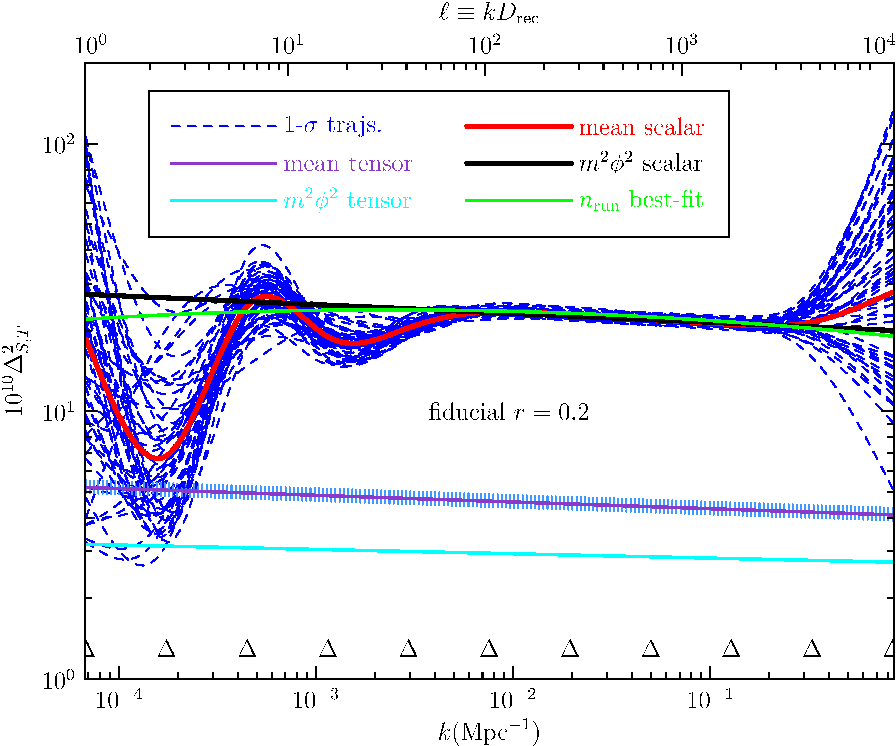
\includegraphics[width=\halffigwidth]{nobicep_spline0_p11_r0d2_power_traj.pdf}%
  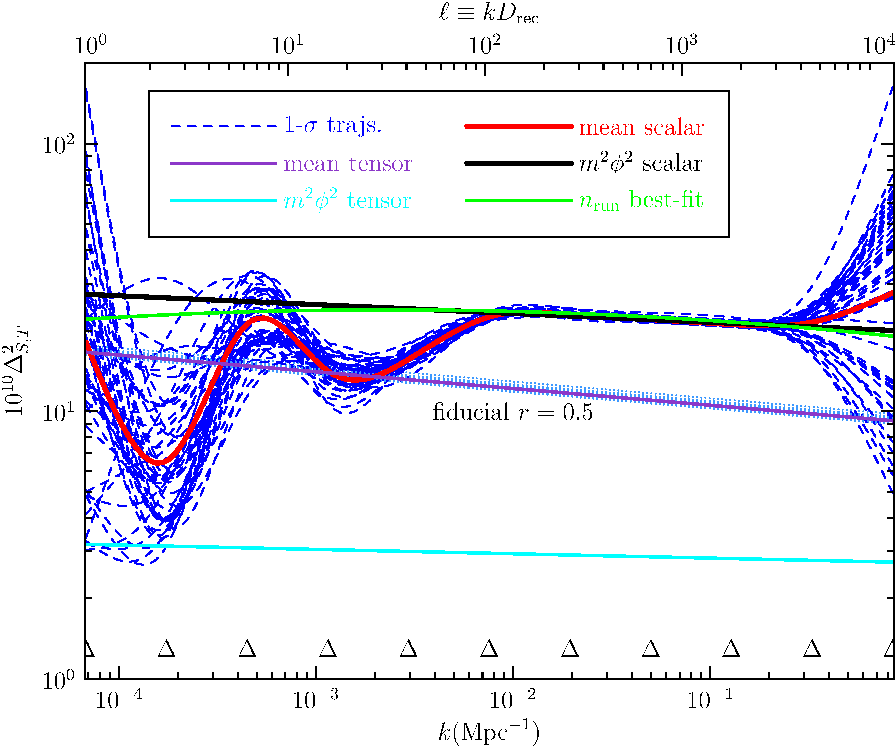
\includegraphics[width=\halffigwidth]{nobicep_spline0_p11_r0d5_power_traj.pdf}
  \caption{Reconstructed power spectra with fiducial $r = 0.02$, $r=0.1$, $r=0.2$, and $r=0.5$ for top-left, top-right, bottom-left, bottom-right panels, respectively. The location of 11 knots used for interpolation are marked with $\Delta$ symbols. Data: Planck + WP + highL + BAO. \label{fig:traj_power_fixr}}
\end{figure}


Due to the aformentioned degeneracy in the temperature data, if we allow $r$ to vary, the reconstructed scalar power spectrum will be driven by the prior in $r$. Do we have a well motivated prior for $r$? A standard approach in the literature is to use a uniform prior on $r$. This prior has a theoretical motivation {\it only if we assume large-field inflations}. Other pirors such as uniform $\ln r$ or $\sqrt{r}$ are entirely possible if we allow a variety of inflation models. Given that we do not really know the order of magnitude of $r$, it is only possible to discuss the reconstruction of scalar power spectrum under an explicit assumption of $r$ or with other indepedent measurement of $r$ to break the degeneracy. In particular, $r$ can be independently measured using the $B$-mode polarization data. We use the currently available BICEP2 $B$-mode polarization data as an example to show how an independent measurement of $r$ can affect the reconstruction of scalar power spectrum. In Fig~\ref{fig:traj_bnb} we compare the reconstructed power spectra for a flat $0\le r \le 1$ prior, with and without BICEP2. Without BICEP2 constraint, the tensor power spectrum can rise up: $r < 0.60$ at 95.4\% confidence level (CL). This is for the standard 11 knots case. The more degrees of freedom we put into the scalar power spectrum, the better the scalar power deficit can mimic the shape shown in Fig~\ref{fig:effps} and the stronger the degeneracy is. As we increase the number of knots to 15, the upperbound becomes even larger: $ r < 0.65$ at 95.4\% CL. 

\begin{figure}
  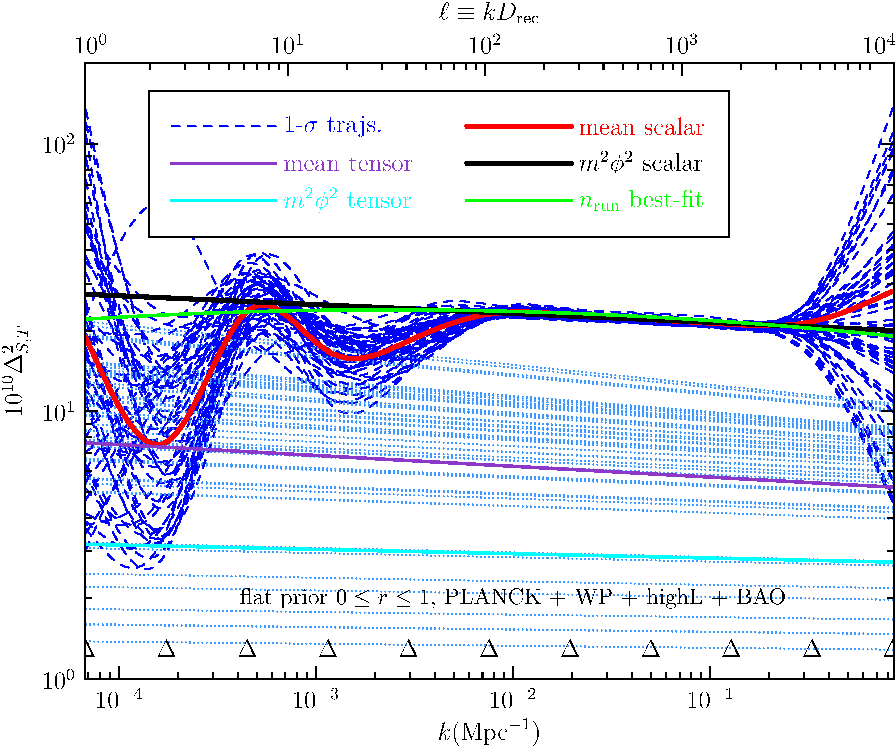
\includegraphics[width = \halffigwidth]{nobicep_spline0_p11_power_trajs.pdf}%
  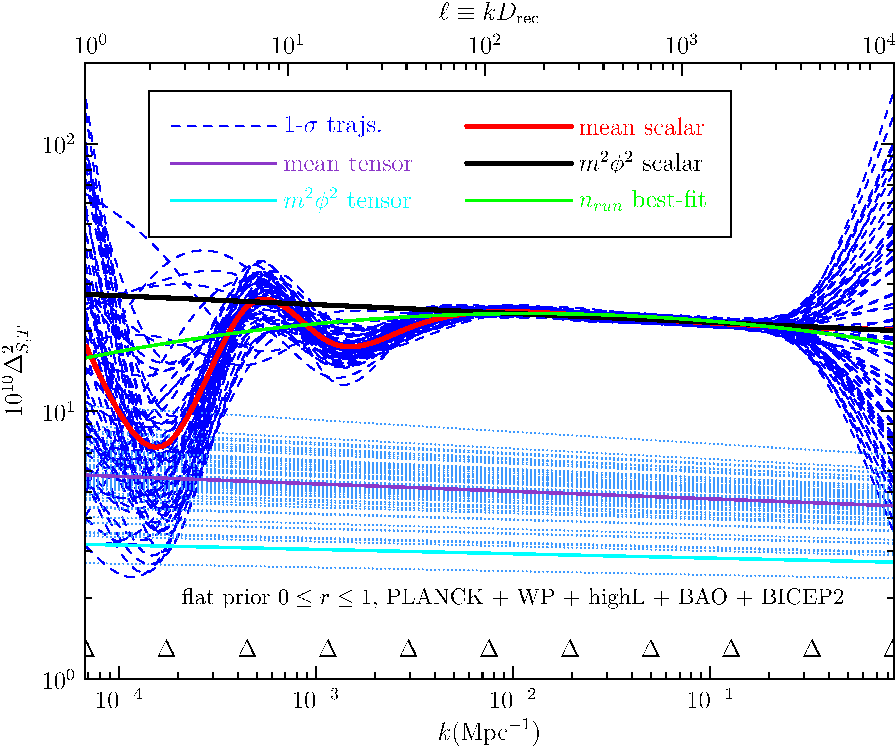
\includegraphics[width = \halffigwidth]{spline0_p11_power_trajs.pdf}
\caption{Reconstructed power spectra with flat prior $0\le r\le 1$: no BICEP2 (left panel) against BICEP2 (right panel). The location of 11 knots used for interpolation are marked with $\Delta$ symbols. Common data sets: Planck + WP + highL + BAO. \label{fig:traj_bnb}}
\end{figure}


Although the reconstructed scalar power spectra differ significantly for different assumptions about the tensor power, we find that, due to the degeneracy between scalar and tensor contributions, the total $C_\ell^{TT}$ remain similar in all cases (fixed fiducial $r$'s and flat prior $r$ with and without BICEP2). In Fig~\ref{fig:traj_cls} we show the similarity of the reconstructed $C_\ell^{TT}$ and the difference in $C_{\ell}^{BB}$, for the cases of flat prior $0\le r \le 1$ with and without BICEP2 constraint. 

\begin{figure}
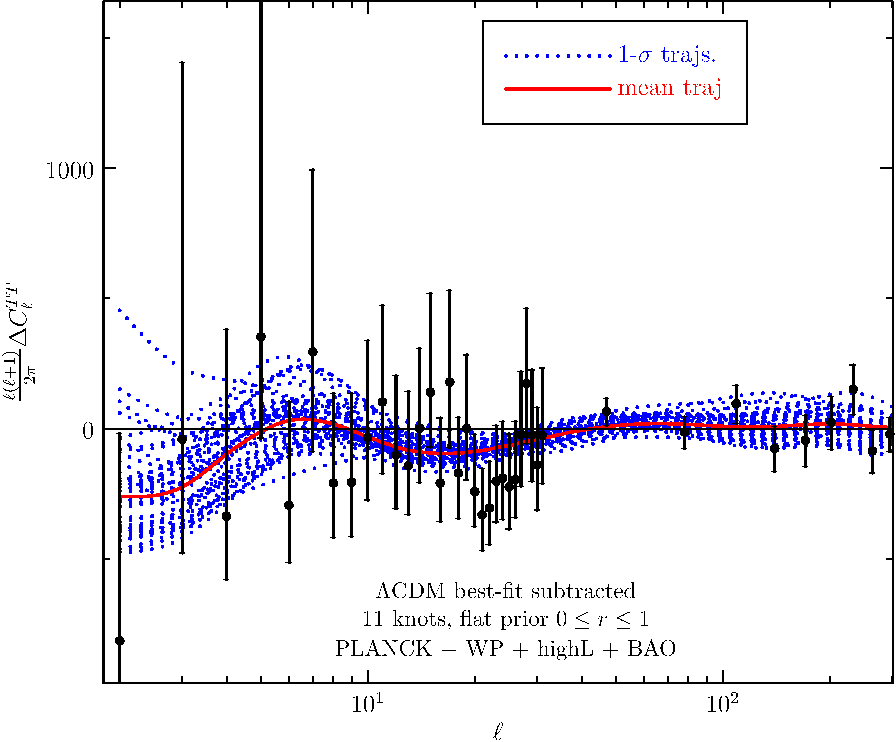
\includegraphics[width = \halffigwidth]{nobicep_spline0_p11_dclTT_trajs.pdf}%
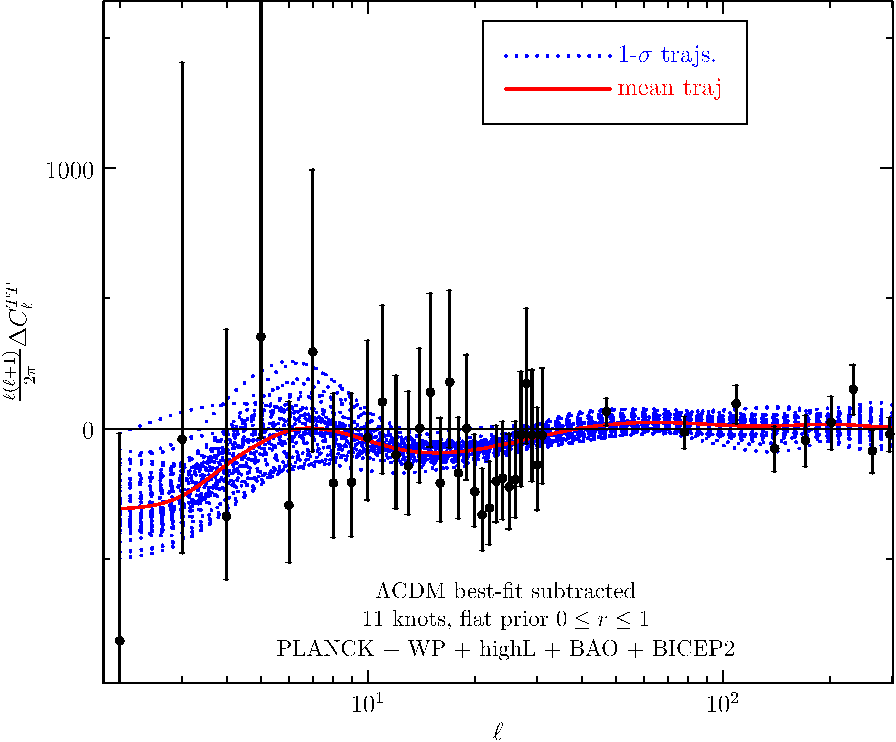
\includegraphics[width = \halffigwidth]{spline0_p11_dclTT_trajs.pdf}
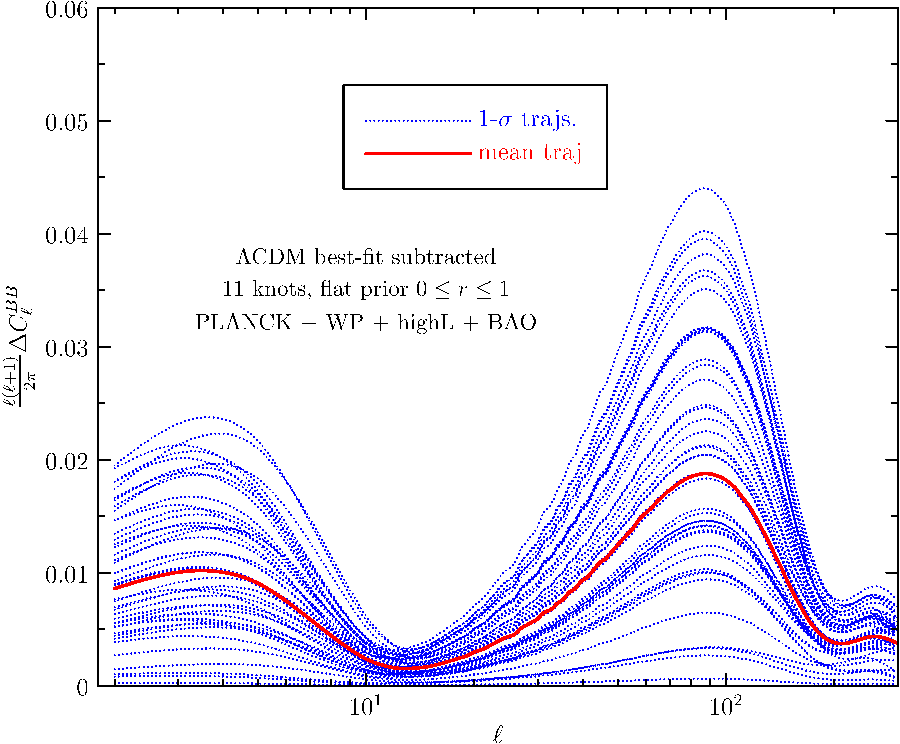
\includegraphics[width = \halffigwidth]{nobicep_spline0_p11_dclBB_trajs.pdf}%
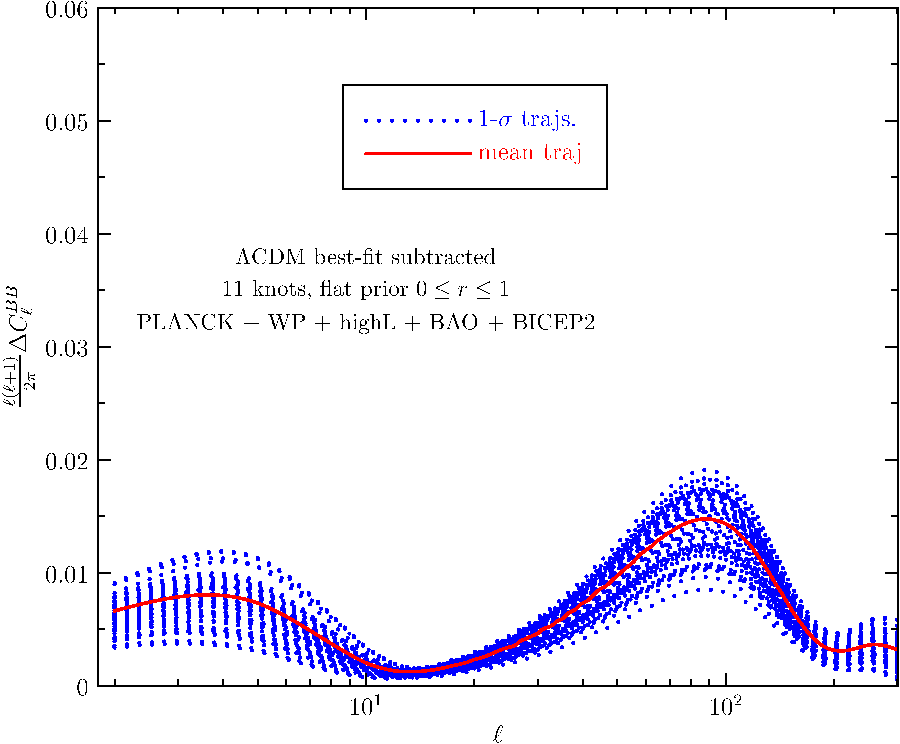
\includegraphics[width = \halffigwidth]{spline0_p11_dclBB_trajs.pdf}
\caption{Reconstructed $C_\ell$ trajectories with $\Lambda$CDM best-fit subtracted: no BICEP2 (left panels) against BICEP2 (right panels). In all panels we have used a flat prior $0\le r\le 1$ and Planck + WP + highL + BAO data.  \label{fig:traj_cls}}
\end{figure}


\section{The low-$\ell$ Power Deficit \label{sec:anomaly}}

Planck reported a tension between the Planck best-fit $\Lambda$CDM model and the low-$\ell$ spectrum in the form of a power deficit of $5$-$10$\% at $l\lesssim 40$, with a statistical significance of $2.5$-$3\sigma$~\cite{Planck2013PowerSpectra}. The Planck analysis used a modified Hausman test, where the lower-bound $\ell_{\min}$ is fixed to be $2$ and the contributions from the proximy of upper-bound $\ell_{\max}$ are filtered by a smoothly damping window. Thus, the exact $\ell$ range contributing to the anomaly has not been identified in details. Here we use a different and more intuitive way to identify the anomaly $\ell$-range.


In Fig~\ref{fig:dcls} Planck $C_\ell^{TT}$ data are plotted against the best-fit $\Lambda$CDM (without BICEP2 constraint) and $\Lambda$CMD~+~$r$ (with BICEP2 constraint) models to demonstrate the low-$\ell$ power deficit anomaly. A coherent power deficit between $\ell=20$ and $\ell = 30$ can be easily identified by eye. The $C_{\ell}$ data are not perfectly uncorrelated at low-$\ell$, making the understanding of the anomaly sophisticated. However, we can assume a full-sky cosmic-variance limited experiment for an order-of-magnitude estimation. Once an analytic understanding of the anomaly is achieved, we proceed with a more exact MCMC calculation.

\begin{figure}
  \centering
  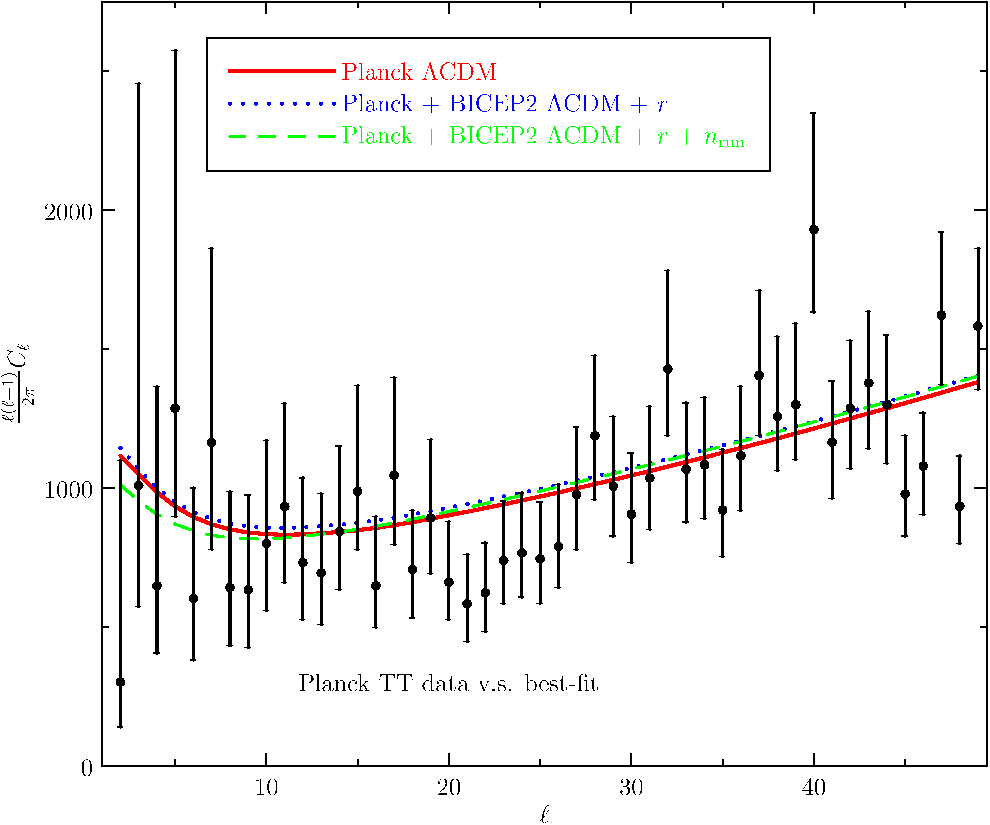
\includegraphics[width =\figwidth]{dcl.pdf}
  \caption{The Planck low-$\ell$ temperature data compared to predictions from various best-fit models. \label{fig:dcls}}
\end{figure}


We can approximately consider the observed $C_\ell$ above or below the model predicted ensemble average as a random binary event for each $\ell$. The probability of seeing $m$ cotinuous identical bits in a sequence of $n$ random bits, $P(m, n)$, can be computed using $P(m, 0) = P(m, 1) = P(m, 2) = \ldots = P(m, m-1) = 0$, $P(m, m) = 1/2^{m-1}$ and the recurrence relation $P(m, n+1 ) = P(m, n) + (1-P(m, n-m))/2^m$ ($n\ge m$). If we take about $100$ multipoles as ``low-$\ell$'', the probability of seeing the $20\le \ell \le 30$ power deficit is then about $P(11, 100)\approx 4\%$. So far we have not taken into account the amplitude of the power deficit. Assuming a coherent power deficit is already seen, the probability of seeing a weighed mean power deficit that is at least as large as the observed one, approximated using the central limit theorem, is 
\begin{equation}
  P = \frac{1}{2}{\rm Erfc}\left[\frac{\sum_{\ell = \ell_{\min}, \ell_{\max}} (2\ell+1)\left(  1 - \sqrt{\frac{4}{\pi(2\ell+1)}} -  \frac{C_\ell^{\rm data}}{C_\ell^{\rm model}}\right)}{2\sqrt{\left(1-\frac{2}{\pi}\right)(\ell_{\max}-\ell_{\min}+1)(\ell_{\max}+\ell_{\min}+1)}}\right] \, .
\end{equation}
Here $C_\ell^{\rm data}$ is the planck temperature power spectrum and $C_\ell^{\rm model}$ is computed for a theoretical model. For the anomaly we are interested in ($\ell_{\min} = 20$ and $\ell_{\max}=30$), the results are P = 55\% for the best-fit $\Lambda$CDM model (without BICEP2 constraint) and P = 31\% for the best-fit $\Lambda$CDM + $r$ model (with BICEP2 constraint). Combining the above discussions, we conclude that the $20\le\ell\le 30$ power deficit is a $\sim 2\%$ rare event for Planck best-fit $\Lambda$CDM model, and a $\sim 1\%$ rare event for Planck~+~BICEP2 best-fit $\Lambda$CDM~+~$r$ model. 

In practice the low-$\ell$ data are correlated and the above estimation may not be accurate. To study the anomaly more rigorously, we use a ``dip parameter'' $A_{\rm dip}$ to phenomenologically describe a power deficit between $\ell_{\min}$ and $\ell_{\max}$. We take the model to be $\Lambda$CDM + $r$ + $n_{\rm run}$ so that we can see whether a running or a power deficit is more preferred by the data. The input $C_{\ell}$ in the likelihood code is $C_\ell^{\rm model}e^{-A_{\rm dip}}$ if $\ell_{\min}\le \ell \le \ell_{\max}$ and $C_\ell^{\rm model}$ otherwise. We have tried various $\ell$ ranges. A full list of the $\ell$ ranges and the corresponding marginalized constraints on $n_{\rm run}$ and $A_{\rm dip}$ are listed in Table~\ref{tbl:nrunadip}. A power deficit is favored by the data for $20\le \ell \le 30$ at $3$-$\sigma$ level and for $2\le \ell \le 30$ at 2.7-$\sigma$ level. We see that in the very-low-$\ell$ range ($2\le \ell \le 19$ or even lower $2\le \ell \le 8$ ) the data do not really favor a coherent deficit against a running, whereas for $20\le\ell\le30$ the data do. This is consistent with Fig~\ref{fig:dcls}. The very-low-$\ell$ data on average, however, are still lower than the $\Lambda$CDM prediction. Including the very-low $\ell$'s for the power deficit does help to relax $n_{\rm run}$ toward zero. To demonstrate the degeneracy between $n_{\rm run}$ and $A_{\rm dip}$ for various choices of $\ell_{\min}$ and $\ell_{\max}$, we show the 1-$\sigma$ and 2-$\sigma$ constraints in the $n_{\rm run}$-$A_{\rm dip}$ space in Fig~\ref{fig:nrunadip}. 

\begin{figure}
  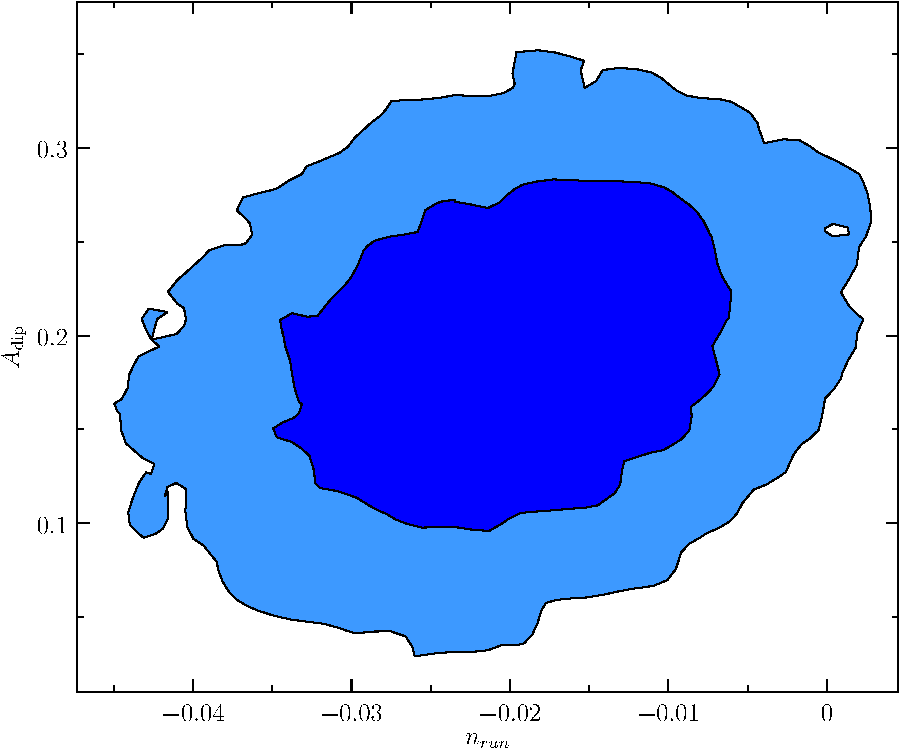
\includegraphics[width = \halffigwidth]{ldip20to30_nrun_dipamp_2D.pdf}%
  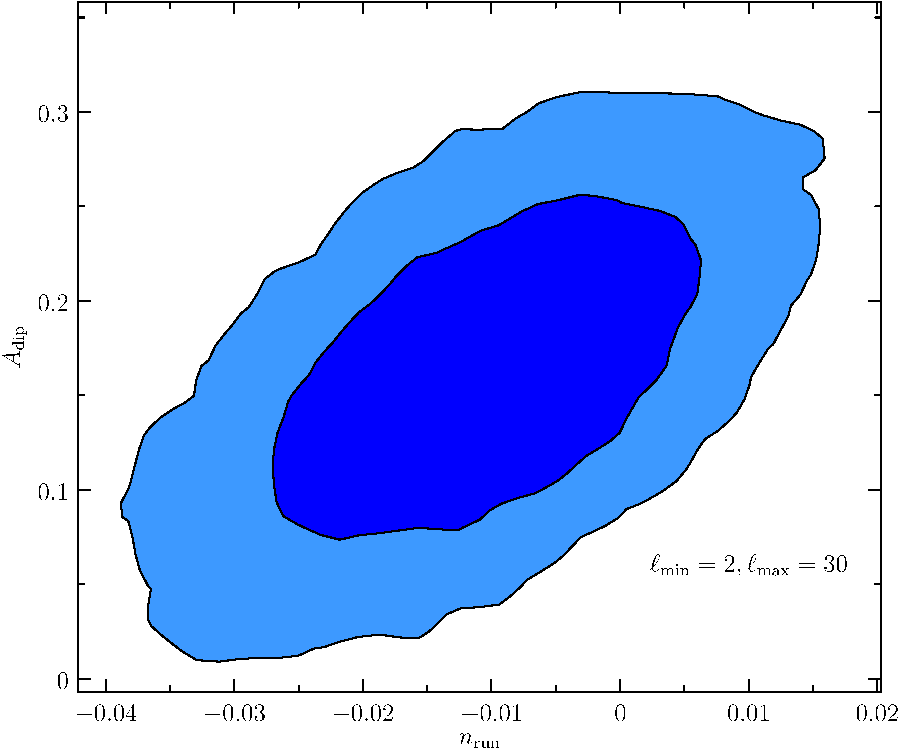
\includegraphics[width = \halffigwidth]{ldip2to30_nrun_dipamp_2D.pdf}
  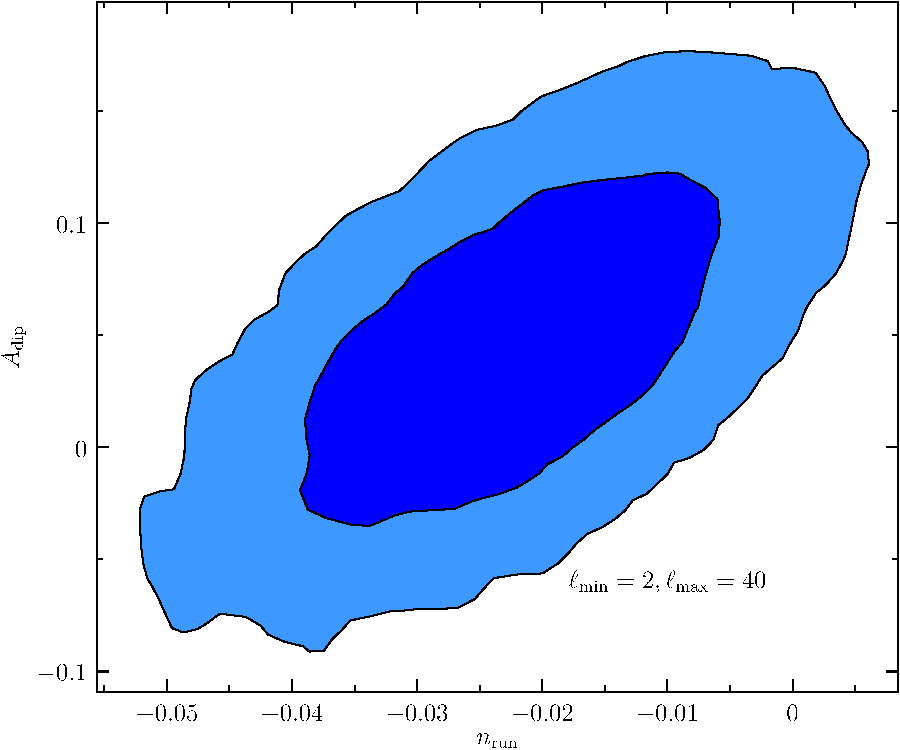
\includegraphics[width = \halffigwidth]{ldip2to40_nrun_dipamp_2D.pdf}%
  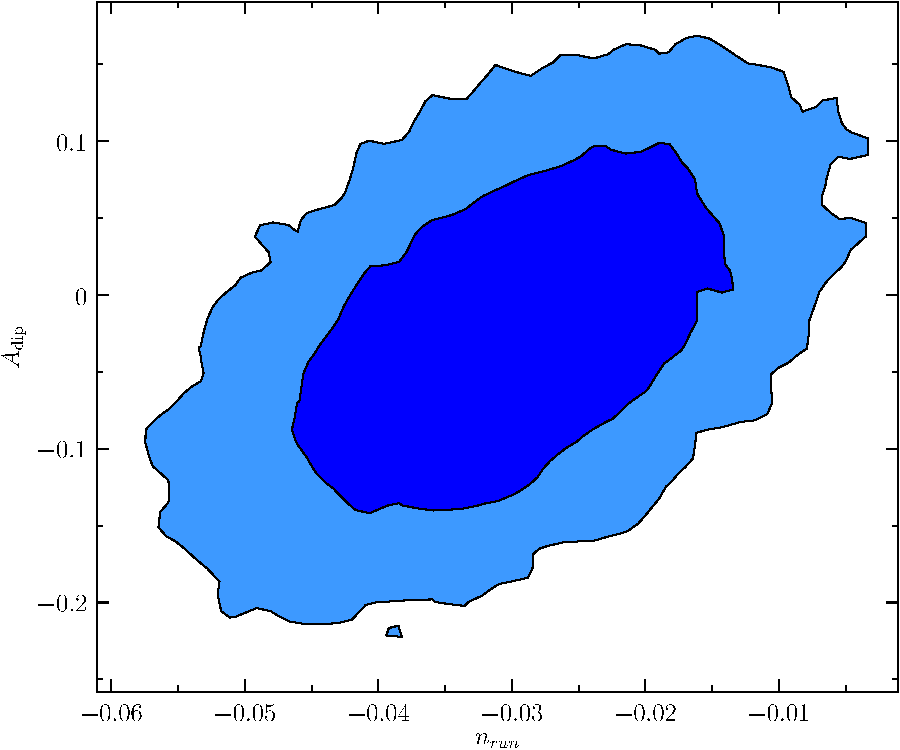
\includegraphics[width = \halffigwidth]{ldip2to19_nrun_dipamp_2D.pdf} 
  \caption{The 68.3\% CL and 95.4\% CL constraints on $n_{\rm run}$ and $A_{\rm dip}$ for the phenomenological power deficit model. The $\ell$ ranges are: top-left panel 20-30;  top-right panel 2-30; lower-left panel 2-40; lower-right panel 2-19. Data sets: Planck + WP + highL + BICEP2 + BAO. \label{fig:nrunadip}}
\end{figure}


\begin{table}
\caption{Margiinalized 95.4\% CL constraints on $n_{\rm run}$ and $A_{\rm dip}$ \label{tbl:nrunadip}}
\centering
\begin{tabular}{ccccc}
\hline
\hline
$\ell_{\min}$ & $\ell_{\max}$ & $n_{\rm run}$ & $A_{\rm dip}$ & significance of $A_{\rm dip}>0$\\
\hline
none & none & $-0.028^{+0.016}_{-0.017}$ & none & none \\
20   & 30 & $-0.020^{+0.016}_{-0.018}$ & $0.18^{+0.12}_{-0.11}$ & $3\sigma$\\
2 & 8 & $-0.030^{+0.017}_{-0.018}$  & $-0.08^{+0.25}_{-0.27}$ & none \\
2 & 19 & $-0.030^{+0.019}_{-0.020}$ &    $-0.02^{+0.15}_{-0.15}$ & none \\
2 & 30 &  $-0.011^{+0.020}_{-0.020}$   & $0.16^{+0.12}_{-0.12}$ & $2.7\sigma$\\
2 & 40 & $-0.023^{+0.021}_{-0.022}$  &  $0.04^{+0.10}_{-0.10}$ & none \\
31 & 50 & $-0.031^{+0.016}_{-0.017}$  & $-0.049^{+0.084}_{-0.085}$ & none\\
51 & 80 & $-0.021^{+0.018}_{-0.021}$  & $0.053^{+0.070}_{-0.067}$ & none\\
\hline
\end{tabular}
\end{table}

\section{Implications for Single-field Inflation Models}

Assuming the underlying physics is single-field inflation, we can reverse-engineer the scalar and tensor power spectra to obtain the expansion history $\epsilon \equiv -\dot H/ H^2$ and the inflaton potential $V(\phi)$. To the lowest order, the reconstruction is

\begin{eqnarray}
  \epsilon(k) & \approx & \frac{\Delta^2_T(k)}{16\Delta^2_S(k)} \, , \\
  \phi(k) & \approx & \phi_{\rm pivot} \pm M_p\int^k_{k_{\rm pivot}} \sqrt{2\epsilon(k')} \frac{dk'}{k'}\, , \label{eq:phirec} \\
  V(k) & \approx & V_{\rm pivot}e^{\int^k_{k_{\rm pivot}} 2\epsilon(k') \frac{dk'}{k'}}\, ,
\end{eqnarray}
where $\phi_{\rm pivot}$ and $V_{\rm pivot}$ are the field and potential values when the pivot mode $k_{\rm pivot} = 0.05 {\rm Mpc}^{-1}$ exits the horizon. The choice of $\phi_{\rm pivot}$ and $\pm$ in eq.~\eqref{eq:phirec} is arbitrary and is just a matter of redefining the field. We use $+$ sign convention so that larger $\phi$ corresponds to larger wavenumber $k$ and smaller scales. The pivot potential $V_{\rm pivot}$ can be determined using 
\begin{equation}
V_{\rm pivot} \approx \frac{\left(3-\epsilon(k_{\rm pivot})\right)M_p^4}{16} \Delta^2_T(k_{\rm pivot}) \, .
\end{equation}

We show the reconstructed $\epsilon$ and $\ln V/V_{\rm pivot}$ trajectories in Fig~\ref{fig:traj_eps} and Fig~\ref{fig:traj_potential}. The reconstructions are done using 11 knots. For various cases we have verified that the reconstruction is not senstive to the number of knots by varying the number of knots from 9 to 15. The potential trajectories tend to bend up on large scales (negative $\phi - \phi_{\rm pivot}$). This is caused by the large-scale power deficit discussed in previous sections. 

\begin{figure}
  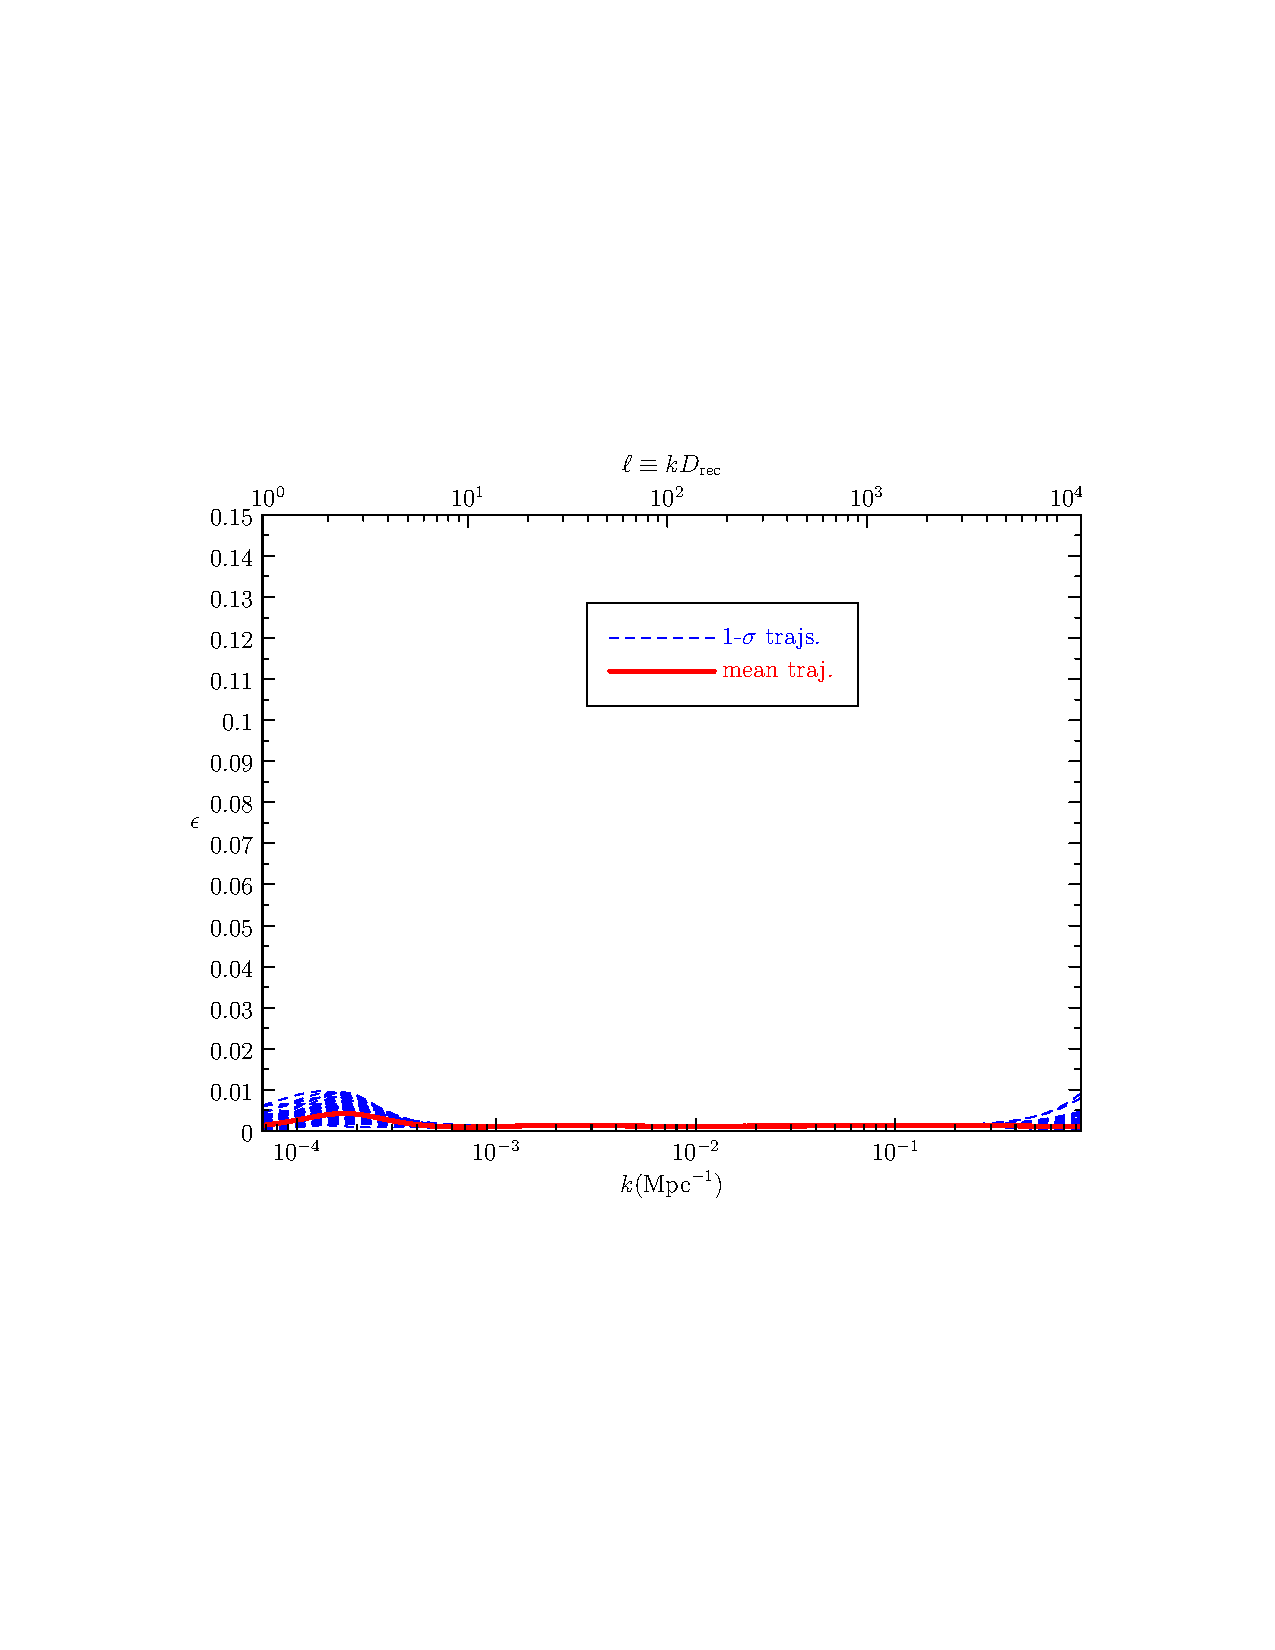
\includegraphics[width=\halffigwidth]{nobicep_spline0_p11_r0d02_eps_traj.pdf}%
  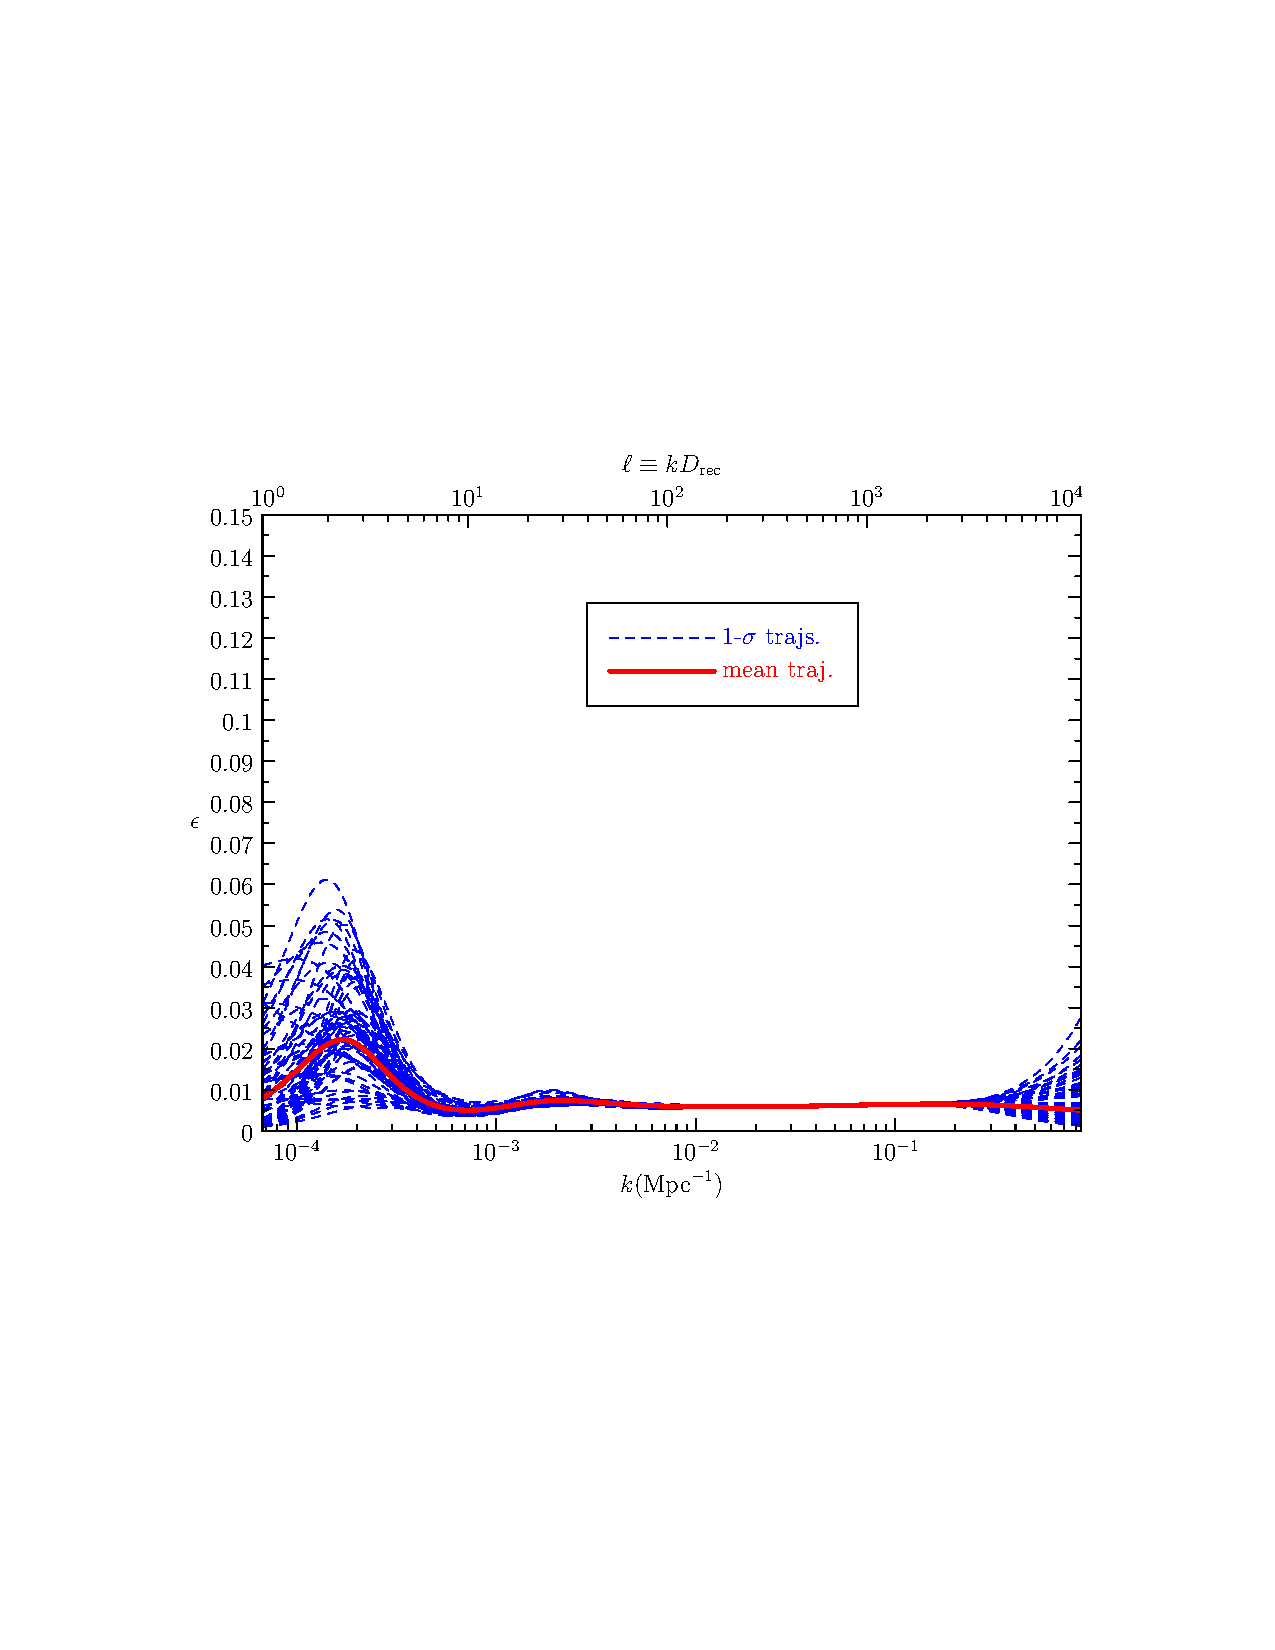
\includegraphics[width=\halffigwidth]{nobicep_spline0_p11_r0d1_eps_traj.pdf} 
  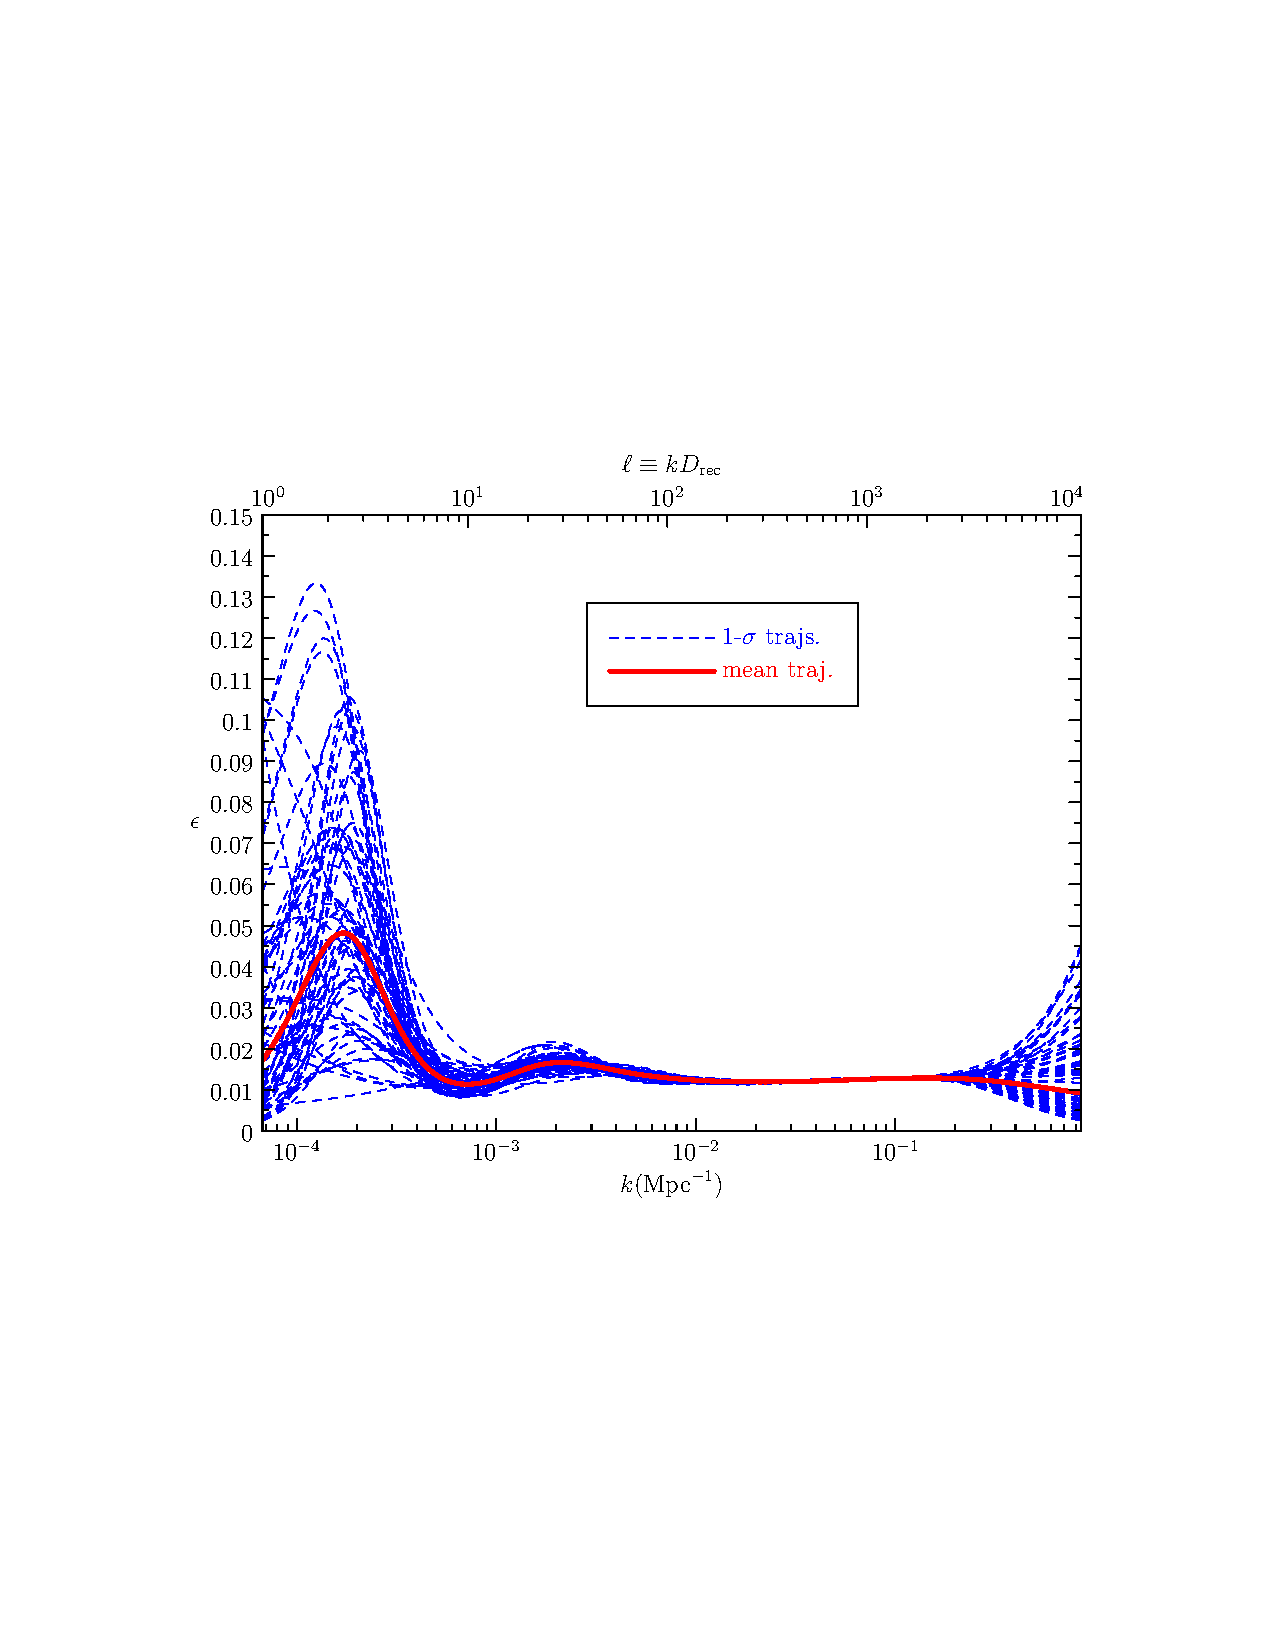
\includegraphics[width=\halffigwidth]{nobicep_spline0_p11_r0d2_eps_traj.pdf}% 
  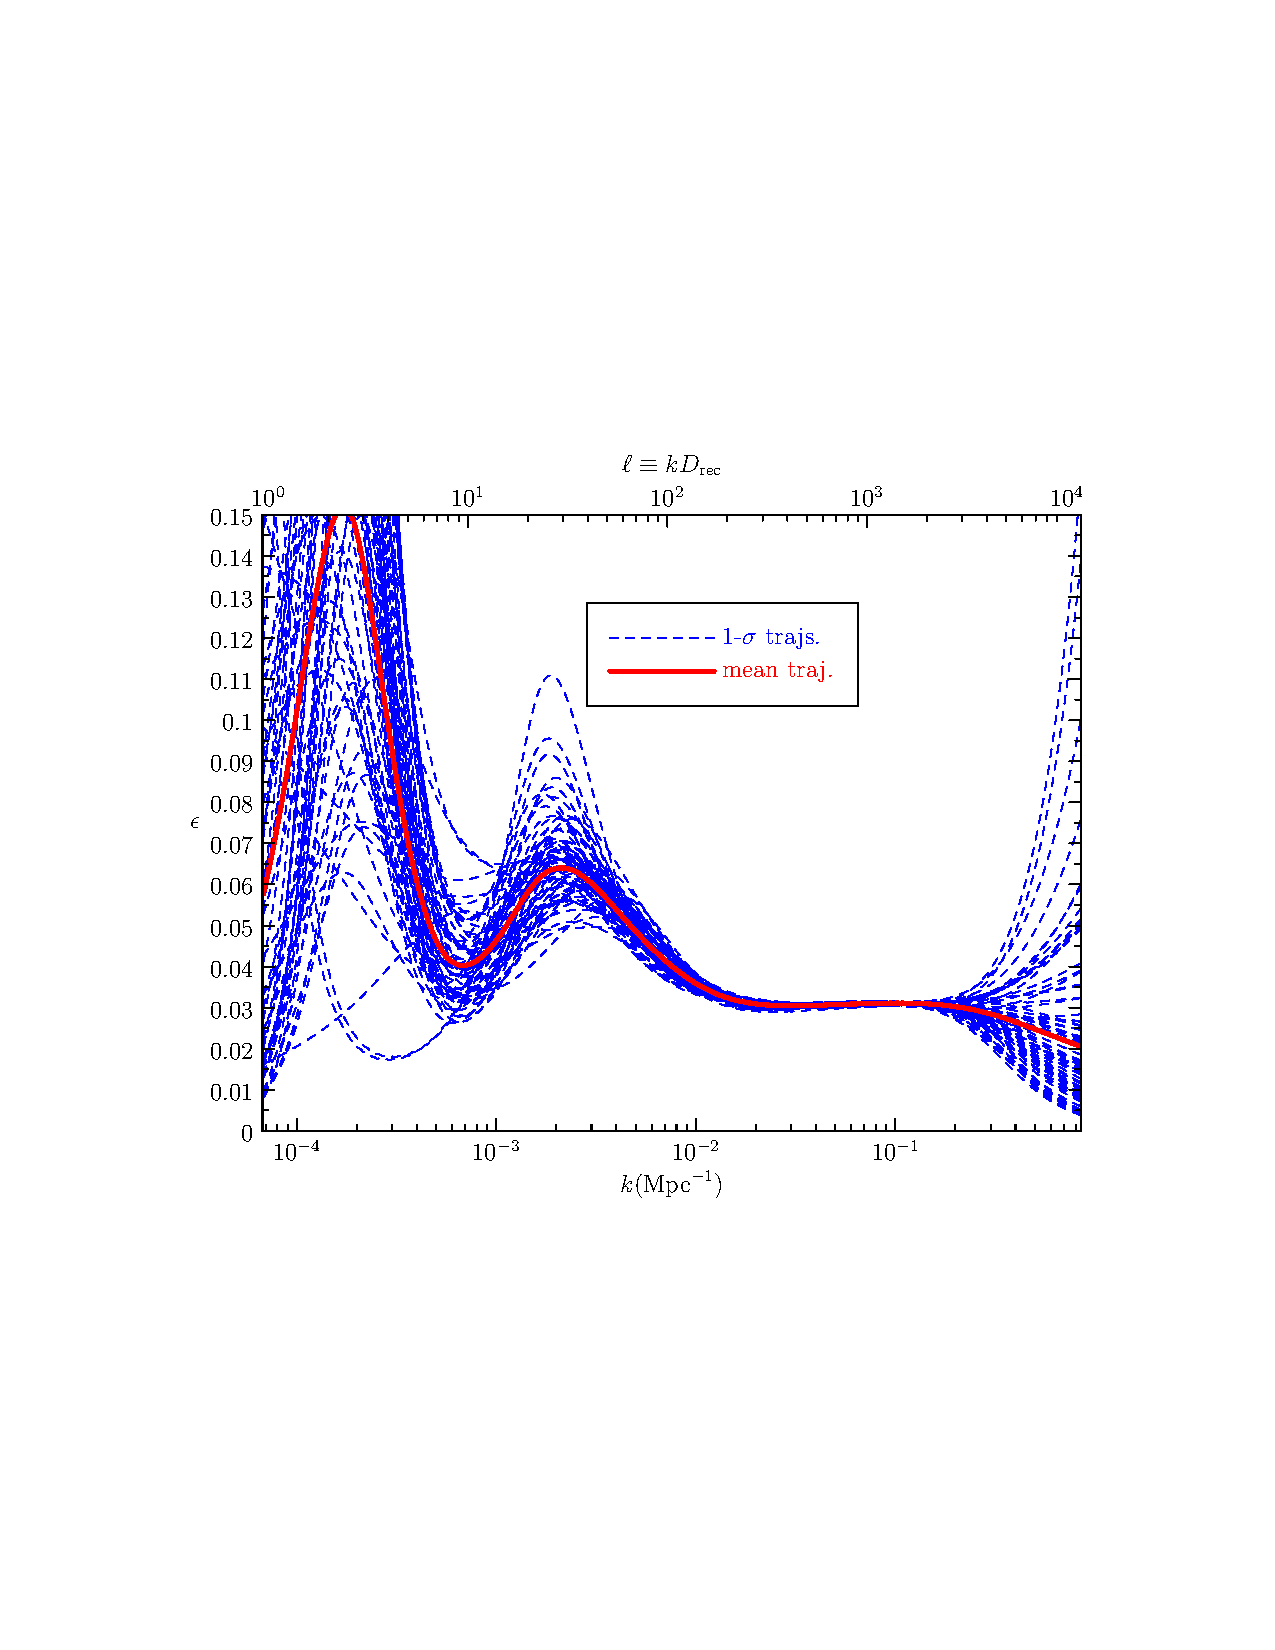
\includegraphics[width=\halffigwidth]{nobicep_spline0_p11_r0d5_eps_traj.pdf}
  \caption{The 11-knots reconstructed $\epsilon$ trajectories with $r = 0.02$, $r=0.2$, $r=0.5$ and free $r$ for top-left, top-right, bottom-left, bottom-right panels, respectively. Data: Planck + WP + highL + BAO. \label{fig:traj_eps}}
\end{figure}


\begin{figure}
  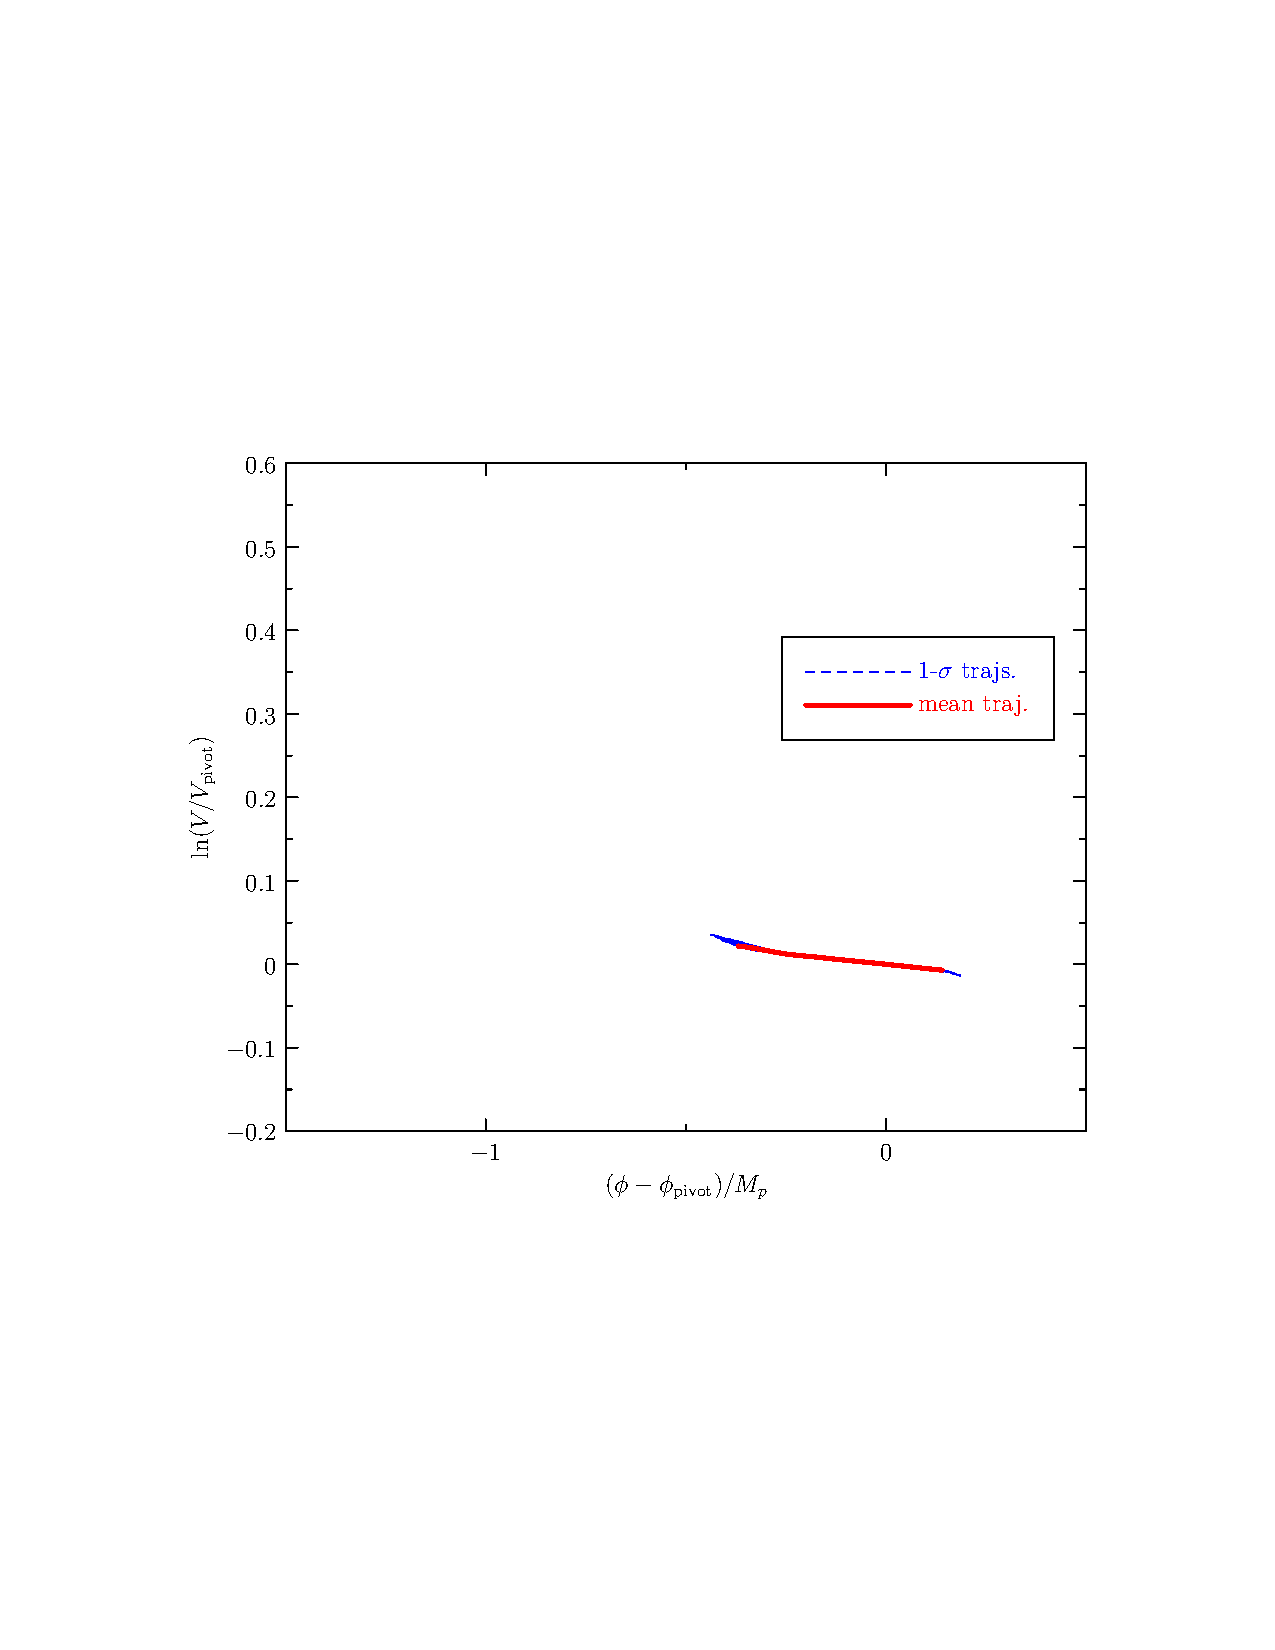
\includegraphics[width=\halffigwidth]{nobicep_spline0_p11_r0d02_potential_traj.pdf}%
  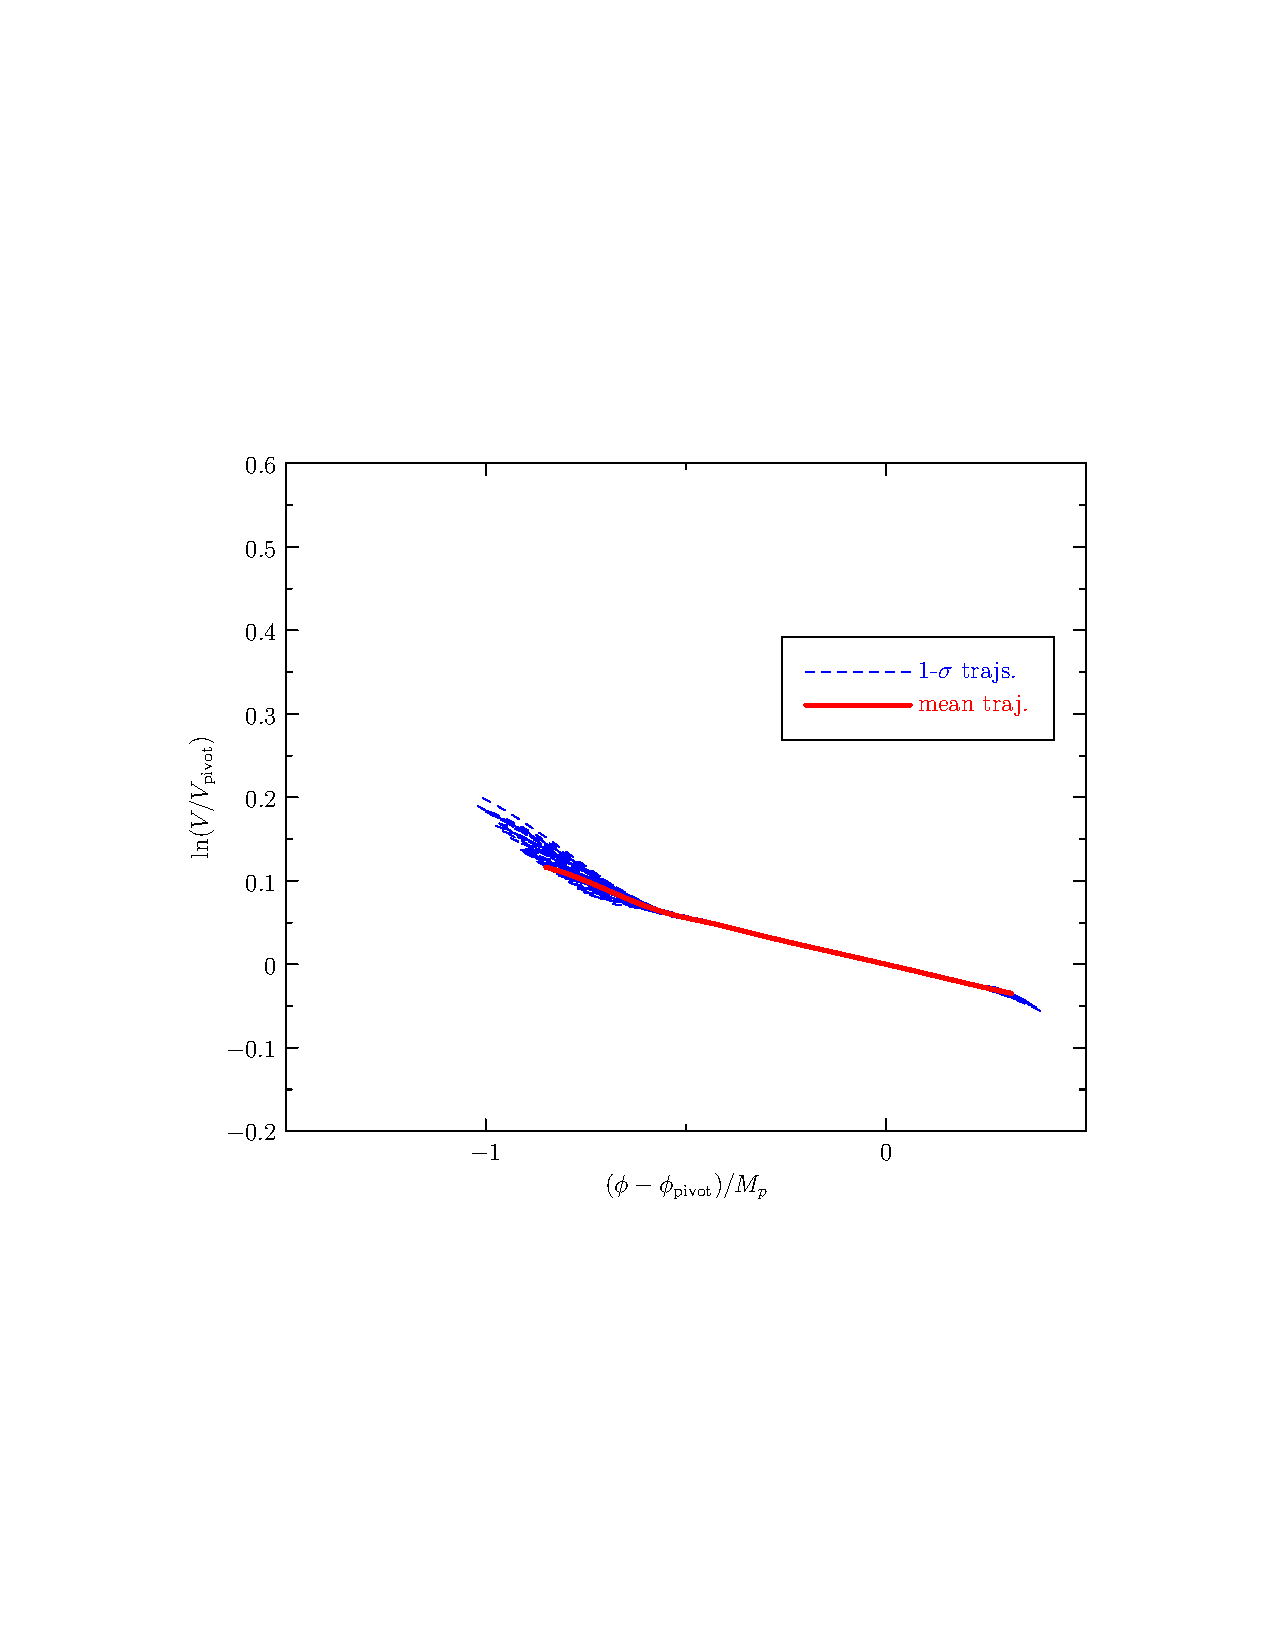
\includegraphics[width=\halffigwidth]{nobicep_spline0_p11_r0d1_potential_traj.pdf} 
  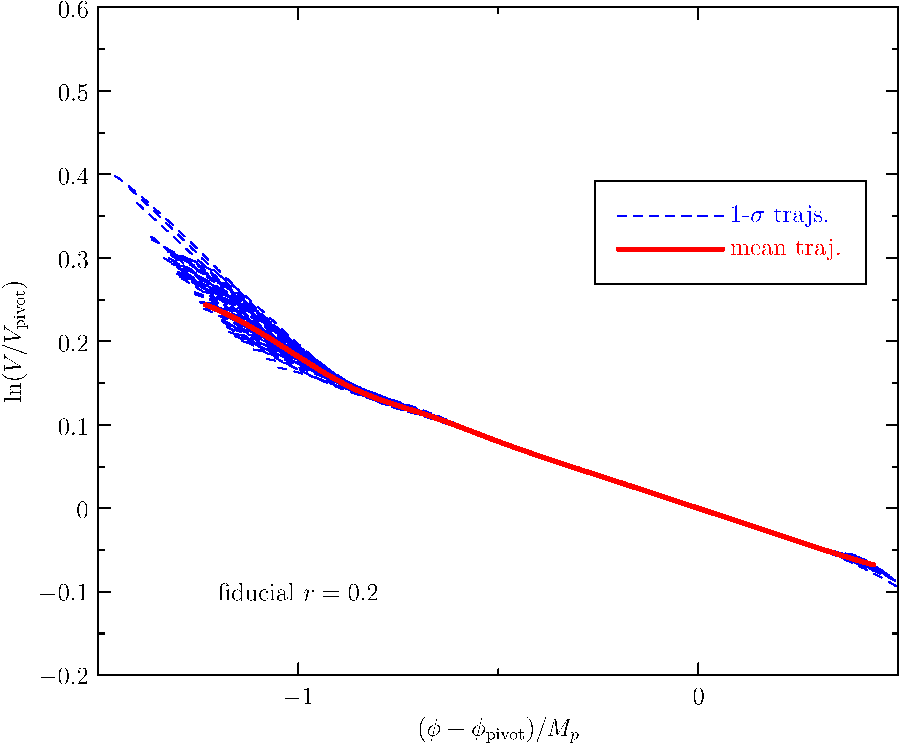
\includegraphics[width=\halffigwidth]{nobicep_spline0_p11_r0d2_potential_traj.pdf}
  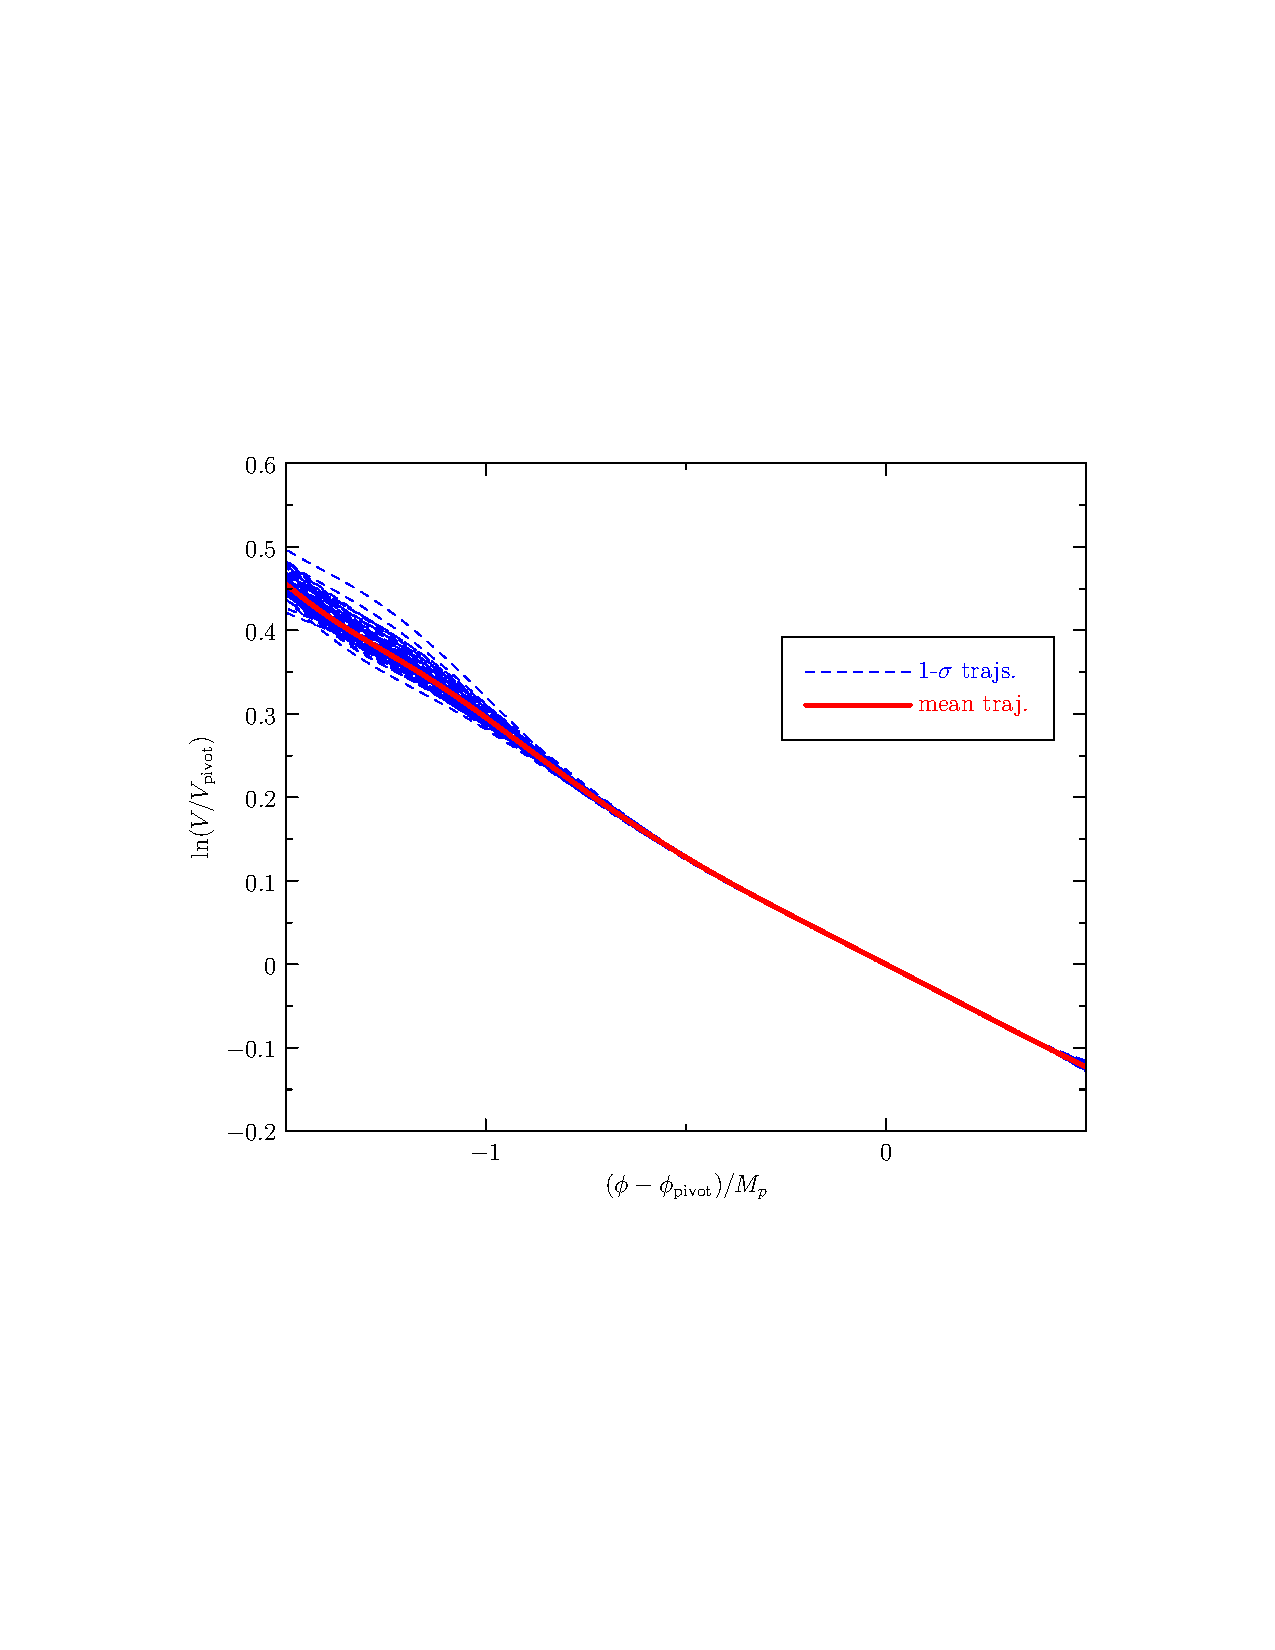
\includegraphics[width=\halffigwidth]{nobicep_spline0_p11_r0d5_potential_traj.pdf}
  \caption{The 11-knots reconstructed potentials with $r = 0.02$, $r=0.1$, $r=0.2$, and $r=0.5$ for top-left, top-right, bottom-left, bottom-right panels, respectively.  Data: Planck + WP + highL + BAO. \label{fig:traj_potential}}
\end{figure}

After all, the purpose of doing the ``model-independent'' reconstruction is to obtain an idea what kind of models the data are driving us towards. The large-scale power deficit drives us to search for a model that allows deviations from power-law scalar power spectrum, where the deviatioins should be
\begin{enumerate}
\item{strongly suppressed on small scales;}
\item{allowing various shapes: simple bending-down, one or two dips, damping oscillations, etc.}
\item{described by very few parameters;}
\end{enumerate}

We find that the step potential model proposed in \cite{Adams2001} have all the above features.
\begin{equation}
V(\phi) = \frac{1}{2}m^2\phi^2\left[1 + \frac{\mu}{2} (1 + \tanh{\frac{\phi - \phi_c}{\delta\phi}}) \right] \,. \label{eq:pot}
\end{equation}
Ref.~\cite{Adams2001} studied the parameter space $\mu \ll 1$ and $\delta\phi \ll M_p$ and found that the scalar power spectrum has damping oscillations. Since the data do not favor any overshooting, the oscillating features may not be a good fit,  at the very least, not obviously better than a running. 

However, if we extend the parameter space to $\mu \lesssim 1$ and $\delta\phi \lesssim 1$, many different new features arise: the scalar power spectrum can have one or two dips without overshooting, or simply bend down to mimic a running. In many cases the deviation from slow-roll is quite significant, it is necessary to use rigorous calculations beyond the slow-roll formalism~\cite{Bardeen1983, Abbott1984,Stewart1993}. We now briefly describe the calculation method and discuss the results.

To map the potential to the scalar and tensor power spectra, we need five parameters: $m$, $\mu$, $\phi_c$, $\delta\phi$ and $N_{\rm inf}$, the number of efolds from the time when $k_{\rm pivot}$ exits the horizon to the end of inflation ($\epsilon = 1$). The standard approach is described in ref.~\cite{Stewart1993}: for each given $k$, one  quantizes the $u_k$ (inflaton field perturbation on spatial-flat gauge) and $v_k$ (tensor metric perturbations) variables and evolve their mode functions till the mode exits the horizon and gets frozen. Numerically, it is not efficient to evolve the mode equations directly, due to its oscillatory nature. In order to achieve a better numeric performance, we split the differential equations of the mode function into an amplitude part and a pahse part. After integrating the phase part analytically, we are left with a single equation describing the evolution of the amplitude of the mode function:
\begin{equation}
  \ddot{\mathcal{A}} + f(t) \dot{\mathcal{A}} + \frac{k^2}{a^2} \mathcal{A} - \frac{e^{-2\int^t f(t) dt}}{\mathcal{A}^3}  = 0, \label{eq:pert}
\end{equation}
where for scalar $f(t) = 3 H - 2 \frac{\dot H}{H} + 2 \frac{\ddot\phi}{\dot\phi}$ for scalar and $f(t) = 3H$ for tensor. 

To solve the euqation eq.~\eqref{eq:pert} one needs to specify the initial conditions. The initial time is chosen such that $aH\ll k$, where the mode is well inside the horizon and the vacuum asympototic solution is $\mathcal{A} \rightarrow \frac{k H }{2\pi a\dot\phi}$ for scalar and $\mathcal{A} \rightarrow \frac{\sqrt{2}k}{\pi a M_p}$ for tensor.  Initial $\dot{\mathcal{A}}$ and the integral constant in $\int^t f(t) dt$ in eq.~\eqref{eq:pert} are fixed by using the initial asymtotic condition.  The final time is chosen such that $aH\gg k$, when the mode is well outside the horizon and $\mathcal{A}$ converges to a constant.  The power spectrum $\Delta^2_{S,T}(k)$ is the square of the converged $\mathcal{A}$. In Fig~\ref{fig:bumppower} we show a few examples of the scalar and tensor power spectra to demonstrate the variety of shapes of scalar power spectrum. 

\begin{figure}
\centering
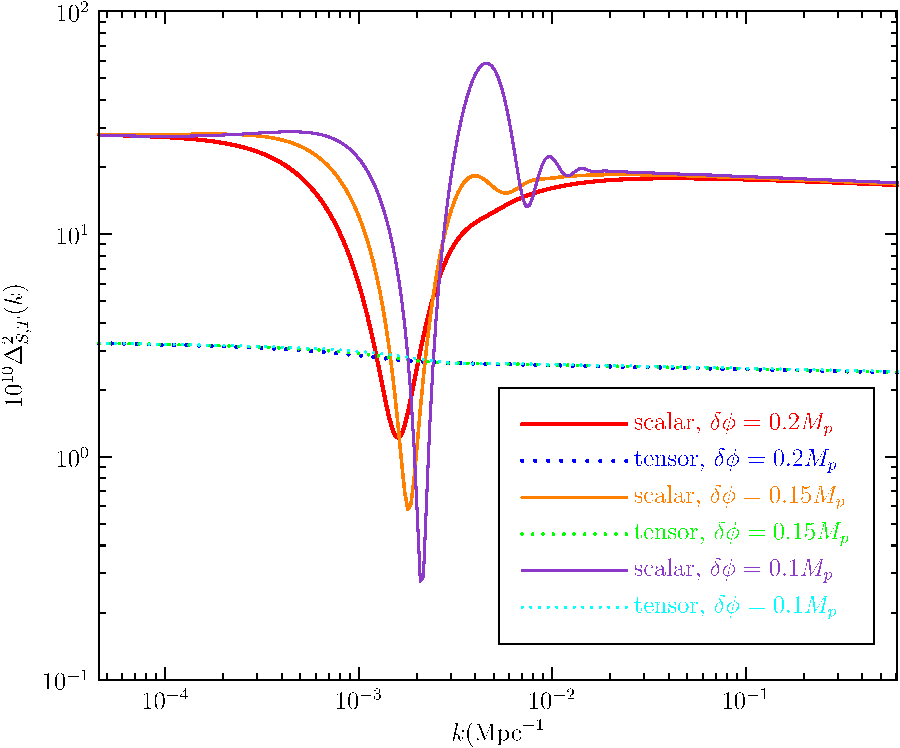
\includegraphics[width=\figwidth]{bumppower.pdf}
\caption{The primordial scalar and tensor power spectra for single-field inflation model defined in eq.~\eqref{eq:pot}. \label{fig:bumppower}}
\end{figure}

For the MCMC run we use flat prior $10^{-6} M_p < m < 10^{-5} M_p$, $0.01 M_p \le \delta\phi\le 0.3 M_p$, $0\le\mu\le 0.5$, $50\le N_{\rm inf} \le 70$. The location of the step, $\phi_c$, is mapped into $\delta N_{\rm step} \equiv \frac{1}{4}(\phi_c^2 - \phi_{\rm pivot}^2)$, which is approximately $ - \ln (k_{\rm step}/k_{\rm pivot})$, $k_{\rm step}$ being the wave number where the dip or osciallating feature is. We use a flat prior $-1 \le N_{\rm step} \le 7$, that is, allowing the feature to be in the range $4.6\times 10^{-5} {\rm Mpc}^{-1} \lesssim k \lesssim 0.14 {\rm Mpc}^{-1}$.

In Fig~\ref{fig:traj_model} we show the posterior power spectra and potential trajctories for this model. Notably, $N_{\rm step}$ is bounded by the data: $N_{\rm step} > 1.2$ at 95.4\% CL, i.e., the scale of the features is at $k<0.015 {\rm Mpc}^{-1}$. 


\begin{figure}
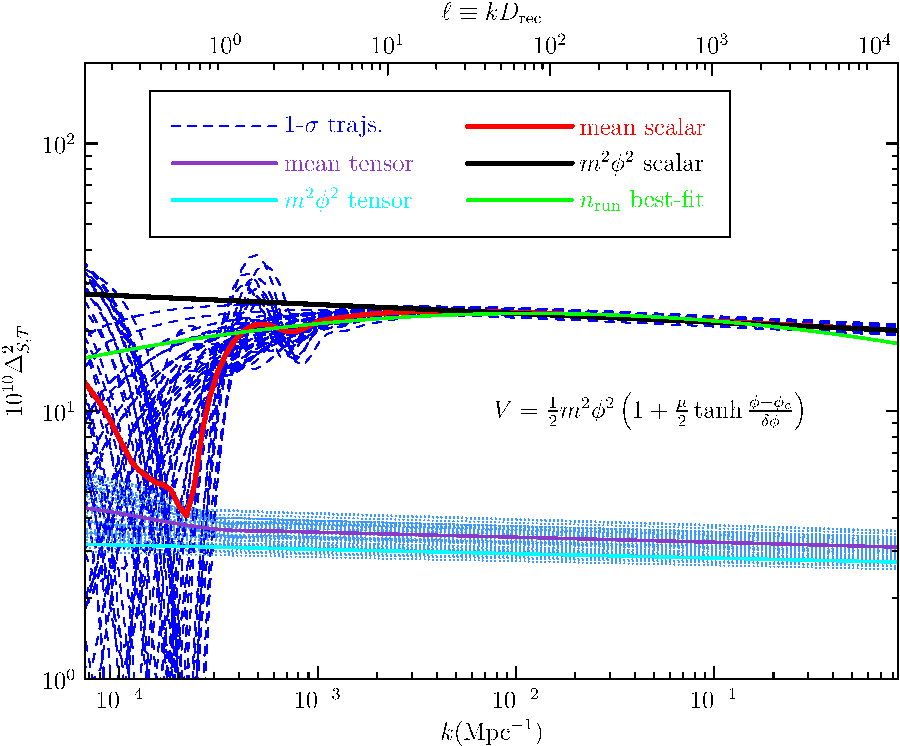
\includegraphics[width=\halffigwidth]{bump_power_trajs.pdf}%
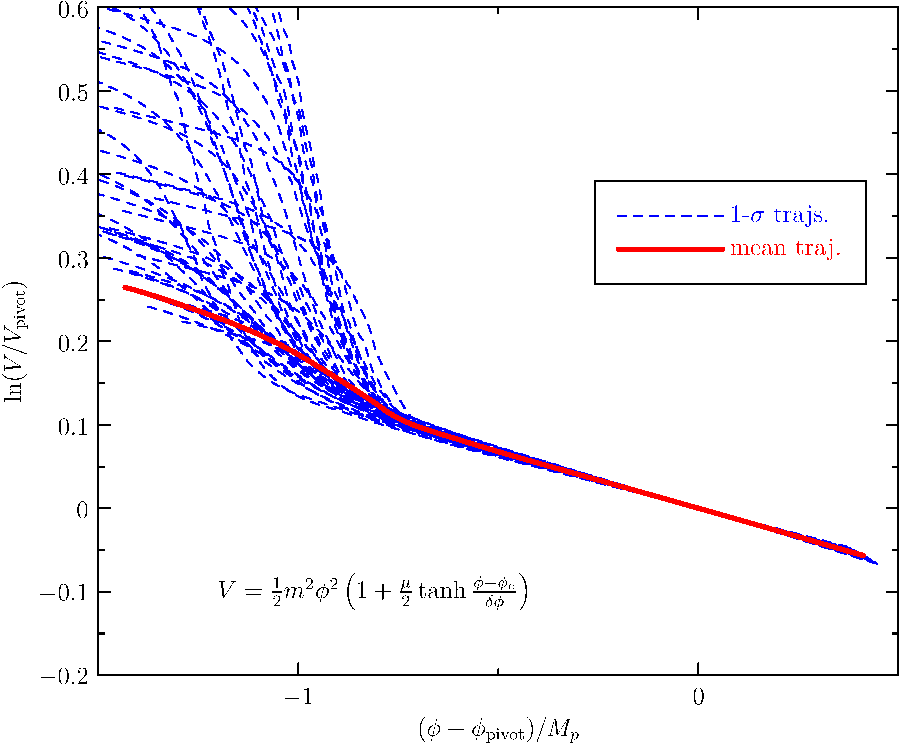
\includegraphics[width=\halffigwidth]{bump_potential_trajs.pdf}
\caption{Reconstructed power spectra and potentials trajectories for the single-field inflation model defined in eq.~\eqref{eq:pot}. Data sets: Planck + WP + highL + BAO + BICEP2. \label{fig:traj_model}}
\end{figure}

\section{Conclusions}

In this paper we studied the bottom-up approach for primordial power spectrum reconstruction. We find that, if only temeprature data is used, the reconstructed scalar power spectrum on large scales ($k\lesssim 0.01 {\rm Mpc}^{-1}$ can be driven by the prior in $r$, due to the degeneracy between scalar and tensor contributions to $C_\ell^{TT}$. We propose explicitly fixing $r$ for the scalar power spectrum reconstructioin, instead of using an {\it ad hoc} prior in $r$ and drawing misleading conclusions. In the presence good-quality polarization data that can break the degeneracy, however, $r$ should be treated as a free parameter.

The reconstructed scalar power deficit on large scales comes with various possible shapes. The spectrum can bend all the way down to superhorizon scales, or have one or two dips. The power deficit is caused by an observed low-$\ell$ power deficit in Planck temperature $C_\ell$ data, which we estimate to be a $\sim 99\%$ CL anomaly. Due to the cosmic variance, the data on large scales do not have sufficient statistical power to measure the detailed shape of the power deficit. Future polarization data and other indepedent cosmological data (such as a large volume galaxy survey) may help to improve the situation.

The simplest single-field inflation models with constant $\epsilon$ are in tension with the scalar power deficit. The large-scale power deficit suggests an up-turning feature in the potential. For parameter study focusing on the power deficit, we propose a simple step potential to accomodate the data without killing variety of possibilities of the shape of the large-scale power deficit.

\section*{Acknowledgements}


\bibliographystyle{JHEP}  
\bibliography{trajectories}



\end{document}
